% documentclass: article used for scientific journals, short reports, program documentation, etc
% options: fontsize 11, generate document for double sided printing, a4-paper
\documentclass[9pt, twoside, a4paper, fleqn]{article}

\usepackage{extsizes}

% package for changing page layout
\usepackage{geometry}
\geometry{a4paper, lmargin=40mm, rmargin=45mm, tmargin=40mm, bmargin=45mm}
% set indentation
\setlength{\parindent}{1em}
% set factor for line spacing
\linespread{1.15}\selectfont
% set (dynamic) additional line spacing
% \setlength{\parskip}{1ex plus 0.5ex minus 0.3ex}

% rigorous formatting (not too much hyphens)
% \fussy
% \sloppy

% package for changing page layout (used to indent whole paragraphs with adjustwidth)
\usepackage{changepage}

% input encoding for special characters (e.g. ä,ü,ö,ß), only for non english text
% options: utf8 as encoding standard, latin1
\usepackage[utf8]{inputenc}
% package for font encoding
\usepackage[T1]{fontenc}
% package for changing used language (especially for more than one language)
% options: ngerman (new spelling) or default: english
\usepackage[ngerman]{babel}
% package for times font
\usepackage{times}
% package for latin modern fonts
% \usepackage{lmodern}

% package for math symbols, functions and environments from ams(american mathematical society)
\usepackage{amsmath}
\usepackage{mathtools}
% package for extended symbols from ams
\usepackage{amssymb}
% package for math black board symbols (e.g. R,Q,Z,...)
\usepackage{bbm}
% package used for calligraphic math symbols
\usepackage{mathrsfs}
% package for extended symbols from stmaryrd(st mary road)
\usepackage{stmaryrd}
% package for more math blackboard symbols
\usepackage{dsfont}

% package defines commands \degree,\celsius for units
\usepackage{gensymb}

% pack­age im­ple­ments scal­ing of the math ex­ten­sion font cmex; used for scaling math signs
\usepackage{exscale}

% package for including extern graphics plus scaling and rotating
\usepackage{graphicx}

% package for positioning figures
\usepackage{float}
% package includes command \FloatBarrier for float-figures; option: section adds barrier for every section, above allows floats to appear above the barrier on the same page
\usepackage[section,above]{placeins}

% package for changing color of font and paper
% options: using names of default colors (e.g red, black)
% \usepackage[usenames]{color}
\usepackage[dvipsnames]{xcolor}
\definecolor{shadecolor}{gray}{0.9}

% package for customising captions
\usepackage[footnotesize, hang]{caption}
% package for subfigures and subcaptions
\usepackage[font=footnotesize]{subcaption}

% package for quotation marks in different languages (use \enquote)
\usepackage[autostyle,german=guillemets]{csquotes}

% package for customising enumerations (e.g. axioms)
\usepackage{enumitem}

% calc package reimplements \setcounter, \addtocounter, \setlength and \addtolength: commands now accept an infix notation expression
\usepackage{calc}

% package for creating framed, shaded, or differently highlighted regions that can break across pages; environments: framed, oframed, shaded, shaded*, snugshade, snugshade*, leftbar, titled-frame
\usepackage{framed}

% package for creating custom "list of"
% options: titles: do not intefere with standard headings for "list of"
\usepackage[titles]{tocloft}

% change enumeration style of equations
% \renewcommand\theequation{\thesection.\arabic{equation}}


% provides \ifthenelse command
\usepackage{ifthen}
% extra commands for if-conditions (e.g. \isempty)
\usepackage{xifthen}

% init list of math for definitions and theorems
\newcommand{\listofmathcall}{Verzeichnis der Definitionen und Sätze}
\newlistof{math}{mathlist}{\listofmathcall}
% add parentheses around argument
\newcommand{\parent}[1]{ \ifx&#1&\else (#1) \fi }
\definecolor{mathdefback}{rgb}{0.95,0.95,0.98}
% unnumerated mathematical definition environment definiton
\newenvironment{mathdef*}[2]{
	\medskip
	\begin{tcolorbox}[colback=mathdefback, boxrule=0.5pt, colframe=black, boxsep=0pt, enhanced jigsaw, breakable, arc=3pt]
	\noindent
	{ \fontfamily{ppl}\selectfont \textbf{\textsc{#1:}} } ~ #2 
	\par \hfill\\ 
	\fontfamily{lmr}\selectfont \itshape
}{
	\end{tcolorbox}
	\medskip
}
% definitions for numerated mathematical definition environment
\newcounter{mathdefc}[section]
\newcommand*{\mathdefnum}{\thesection.\arabic{mathdefc}}
\renewcommand{\themathdefc}{\mathdefnum}
\newenvironment{mathdef}[2]{
	\refstepcounter{mathdefc}
	\addcontentsline{mathlist}{figure}{\protect{\numberline{\mathdefnum}#1 ~ #2}}
	\begin{mathdef*}{#1 \mathdefnum}{#2}
}{
	\end{mathdef*}
}
% standard mathdef calls
\newcommand{\definitioncall}{Definition}
\newenvironment{definition*}[1][]{ \begin{mathdef*}{\definitioncall}{\parent{#1}} }{ \end{mathdef*} }
\newenvironment{definition}[1][]{ \begin{mathdef}{\definitioncall}{\parent{#1}} }{ \end{mathdef} }

\definecolor{maththeoremframe}{rgb}{0.7,0.7,0.73}

% unnumerated theorem environment definition
\newenvironment{maththeorem*}[2]{
	\medskip
	\begin{tcolorbox}[boxrule=0pt, leftrule=2.5pt, arc=2pt, colback=white, colframe=maththeoremframe, enhanced jigsaw, breakable, vfill before first, top=0mm, bottom=0mm, left=2mm, right=0mm, boxsep=1mm]
	\noindent
	{ \fontfamily{ppl}\selectfont \textbf{\textsc{#1:}} } ~ #2
	\par \hfill\\ 
	\fontfamily{lmr} \fontshape{it} \selectfont
}{ 
	\end{tcolorbox}
	\medskip
}
% definitions for numerated theorem environment
\newcounter{maththeoremc}[section]
\newcommand*\maththeoremnum{\thesection.\arabic{maththeoremc}}
\renewcommand{\themaththeoremc}{\maththeoremnum}
\newenvironment{maththeorem}[2]{
	\refstepcounter{maththeoremc}
	\addcontentsline{mathlist}{figure}{\protect{\qquad\numberline{\maththeoremnum}#1 ~ #2}}
	\begin{maththeorem*}{#1 \maththeoremnum}{#2}
}{
	\end{maththeorem*}
}
% standard maththeorem calls
\newcommand{\theoremcall}{Theorem}
\newenvironment{theorem*}[1][]{ \begin{maththeorem*}{\theoremcall}{\parent{#1}} }{ \end{maththeorem*} }
\newenvironment{theorem}[1][]{ \begin{maththeorem}{\theoremcall}{\parent{#1}} }{ \end{maththeorem} }
\newcommand{\lemmacall}{Lemma}
\newenvironment{lemma*}[1][]{ \begin{maththeorem*}{\lemmacall}{\parent{#1}} }{ \end{maththeorem*} }
\newenvironment{lemma}[1][]{ \begin{maththeorem}{\lemmacall}{\parent{#1}} }{ \end{maththeorem} }
\newcommand{\propositioncall}{Proposition}
\newenvironment{proposition*}[1][]{ \begin{maththeorem*}{\propositioncall}{\parent{#1}} }{ \end{maththeorem*} }
\newenvironment{proposition}[1][]{ \begin{maththeorem}{\propositioncall}{\parent{#1}} }{ \end{maththeorem} }
\newcommand{\corollarycall}{Korollar}
\newenvironment{corollary*}[1][]{ \begin{maththeorem*}{\corollarycall}{\parent{#1}} }{ \end{maththeorem*} }
\newenvironment{corollary}[1][]{ \begin{maththeorem}{\corollarycall}{\parent{#1}} }{ \end{maththeorem} }
% q.e.d. definition
\newcommand{\qed}{ \par \hfill \fontfamily{lmr} \fontshape{it} \selectfont \mbox{q.e.d.} \\}
\newcommand{\qedbox}{ \hfill $\Box$ }
% proof environment definition for theorems
\newenvironment{mathproof}[2]{
	% \par\hfill\\
	\medskip
	% \noindent
	% \par
	% { \fontfamily{ppl}\selectfont \small \textsc{#1:} } ~ \parent{#2} \smallskip\\
	% \begin{adjustwidth}{1em}{}
	\begin{tcolorbox}[title= { \fontfamily{ppl}\selectfont \small \textsc{#1:} } ~ \parent{#2}, boxrule=0pt, colback=white, colframe=white, coltitle=black, breakable, boxsep=0mm, top=2mm, bottom=0mm, right=0mm, left=0mm, before upper={\parindent1em}]%
	\normalfont
	\small
}{ 
	\end{tcolorbox}
	% \end{adjustwidth} 
	% \qedbox
	\medskip
}
% standard mathproof calls
\newcommand{\proofcall}{Beweis}
\newenvironment{proof}[1][]{ \begin{mathproof}{\textbf{\proofcall}}{#1} }{ \qedbox \end{mathproof} }
\newcommand{\proofideacall}{Beweisidee}
\newenvironment{proofidea}[1][]{ \begin{mathproof}{\proofideacall}{#1} }{ \end{mathproof} }

% math environment for examples (not numerated)
\newcommand{\examplecall}{Beispiel}
% \newcommand{\examplebox}{\hfill $\blacksquare$}
\newcommand{\examplebox}{\hfill $\rule{5pt}{5pt}$}
% \newenvironment{example}[1][]{ \begin{mathproof}{\examplecall}{#1} }{ \end{mathproof} }
\newenvironment{example}[1][]{
	\medskip
	\normalfont
	\small
	\textsc{\examplecall}: ~ \parent{#1} \\
}{
	% \par
	\examplebox
	\par
	\medskip
}
% fast font types
\newcommand{\m}[1]{\mathrm{#1}}
\newcommand{\s}[1]{\mathcal{#1}}
\newcommand{\e}[1]{\mathscr{#1}}


% logical equivalent define
\newcommand{\logeq}{\mathrel{\vcentcolon\Longleftrightarrow}}


% define
\newcommand{\define}{\coloneqq}
% define sign from the right
\newcommand{\definedby}{\eqqcolon}
% function
\newcommand{\func}[3]{#1\colon#2\to#3}


% brackets
% curly brackets
\newcommand{\curlb}[1]{\left\{ #1 \right\}}
% box brackets
\newcommand{\boxb}[1]{\left[ #1 \right]}
% parentheses/curved brackets
\newcommand{\curvb}[1]{\left( #1 \right)}
% angle brackets
\newcommand{\angleb}[1]{\left\langle #1 \right\rangle}
% floor brackets
\newcommand{\floorb}[1]{\left\lfloor #1 \right\rfloor}
% ceil brackets
\newcommand{\ceilb}[1]{\left\lceil #1 \right\rceil}


% symbols for sets
% create sets
% \newcommand{\set}[2][]{ \curlb{#2 \ifx&#1&\else \enspace\middle\vert\enspace #1 \fi} }
\newcommand{\set}[2][]{ \curlb{#2 \ifthenelse{\isempty{#1}}{}{\enspace\middle\vert\enspace #1}} }
% standard sets
\newcommand{\SR}{\mathds{R}} % real numbers
\newcommand{\SC}{\mathds{C}} % complex numbers
\newcommand{\SN}{\mathds{N}} % natural numbers
\newcommand{\SZ}{\mathds{Z}} % integral numbers
\newcommand{\SQ}{\mathds{Q}} % rational numbers
\newcommand{\SFP}{\mathds{P}} % polynom functions
\newcommand{\SFC}{\mathrm{C}} % complex valued functions (continous or differentiable)
\newcommand{\SFL}{\mathcal{L}} % space of integrable functions
\newcommand{\SFLL}{\mathrm{L}} % space of integrable function classes
% set of linear maps
\newcommand{\LM}{L}
% hilbert space
\newcommand{\SH}{\mathcal{H}}
% set of matrices
\newcommand{\SM}{\mathrm{M}}
% set of invertible
\newcommand{\SGL}{\mathrm{Gl}}
% group of orthogonal matrices
\newcommand{\SO}{\mathrm{O}}
% special group of orthogonal matrices
\newcommand{\SSO}{\mathrm{SO}}
% group of unitary matrices
\newcommand{\SU}{\mathrm{U}}
% hauptraum/generalized eigenspace
\newcommand{\hau}{\mathrm{Hau}}


% elements
% identity
\DeclareMathOperator{\id}{id}
% identity matrix
\newcommand{\idmat}{\mathrm{I}}
% normal distribution
\newcommand{\FN}{\mathcal{N}}


% operators
% inverse
\newcommand{\inv}[1]{ {#1}^{-1} }
% magnitude/absolute value
\newcommand{\abs}[1]{\left\vert #1 \right\vert}
% norm
\newcommand{\norm}[1]{\left\| #1 \right\|}
% power of set
\DeclareMathOperator{\setpow}{\mathcal{P}}
% real part
\DeclareMathOperator{\real}{Re}
% imaginary part
\DeclareMathOperator{\imag}{Im}
% complex conjugate
\newcommand{\conj}[1]{ \overline{#1} }
% diagonal matrix
\DeclareMathOperator{\diag}{diag}
% trace of matrix
\DeclareMathOperator{\tr}{tr}
% kernel of function
% \DeclareMathOperator{\ker}{ker}
% image of function
\DeclareMathOperator{\im}{im}
% annihilator
\DeclareMathOperator{\ann}{ann}
% transponent matrix
\newcommand{\transp}[1]{ {#1}^\m{T} }
% spectrum of matrix
\DeclareMathOperator{\spec}{\sigma}
% rank of matrix
\DeclareMathOperator{\rank}{rank}
% signum of permutation or number
\DeclareMathOperator{\sign}{sgn}
% expectation
\DeclareMathOperator{\expect}{\mathbb{E}}
% variance
\DeclareMathOperator{\var}{var}
% fourier transform
\newcommand{\fourier}{\mathcal{F}}
% derivative
\DeclareMathOperator{\Deriv}{D}
\newcommand{\deriv}[1]{ {#1}^{\prime} }
\newcommand{\dderiv}[1]{ {#1}^{\prime\prime} }
\newcommand{\ddderiv}[1]{ {#1}^{\prime\prime\prime} }
\newcommand{\nderiv}[2][]{ \ifx&#1& \deriv{#2} \else {#2}^{(#1)} \fi }
\DeclareMathOperator{\pderiv}{\partial}
% infinitesimal difference
\newcommand{\diff}{\mathrm{d}}
% integral
\newcommand{\integral}[4]{\int_{#1}^{#2} #3\ \diff #4}
\newcommand{\Integral}[4]{\int\limits_{#1}^{#2} #3\ \diff #4}
\newcommand{\iintegral}[2]{\int #1\ \diff #2} % indefinite integral
% scalar product
\newcommand{\dotp}[2]{\angleb{#1,#2}}
% cross product sign
\newcommand{\cross}{\times}
% cross product function
\newcommand{\crossp}[2]{#1 \cross #2}
% sign for direct sum
\newcommand{\dsum}{\oplus}
% linear span
\newcommand{\lspan}[1]{\angleb{#1}}
% dual space
\newcommand{\dual}[1]{ {#1}^* }
\newcommand{\ddual}[1]{ {#1}^{**} }
% bra-vector
\newcommand{\ket}[1]{ \left| #1 \right\rangle }
% ket-vector
\newcommand{\bra}[1]{ \left\langle #1 \right| }
% bracket
\newcommand{\bracket}[2]{ \left\langle #1 \middle| #2 \right\rangle }
% expectation of operator
\newcommand{\opexpect}[1]{ \angleb{#1} }

% converges arrow
\newcommand{\conv}[1][]{\xrightarrow[]{#1}}


% append unit
\newcommand{\unit}[1]{\, \mathrm{#1}}

% show formal atom with element name
\newcommand{\atom}[3][]{\prescript{#3}{#1}{\m{#2}}}
% show formal atom with variabel as name
\newcommand{\atomv}[3][]{\prescript{#3}{#1}{#2}}



% package for init listings(non-formatted  text) e.g. different source codes
\usepackage{listings}


% definitions for listing colors
\definecolor{codeDarkGray}{gray}{0.2}
\definecolor{codeGray}{gray}{0.4}
\definecolor{codeLightGray}{rgb}{0.94,0.94,0.91}
\definecolor{codeBorder}{rgb}{0.34,0.24,0.21}
% predefinitions for listings
\newcommand{\listingcall}{Listing}
\newlength{\listingframemargin}
\setlength{\listingframemargin}{1em}
\newlength{\listingmargin}
\setlength{\listingmargin}{0.08\textwidth}
% \newlength{\listingwidth}
% \setlength{\listingwidth}{ ( \textwidth - \listingmargin * \real{2} + \listingframemargin * \real{2} ) }
% definitions for list of listings
\newcommand{\listoflistingscall}{\listingcall -Verzeichnis}
\newlistof{listings}{listinglist}{\listoflistingscall}
% style definition for standard code listings
\lstdefinestyle{std}{
	belowcaptionskip=0.5\baselineskip,
	breaklines=true,
	frameround=tttt,
	% frame=false,
	xleftmargin=0em,
	xrightmargin=0em,
	showstringspaces=false,
	showtabs=false,
	% tab=\smash{\rule[-.2\baselineskip]{.4pt}{\baselineskip}\kern.5em},
	basicstyle= \fontfamily{pcr}\selectfont\footnotesize\bfseries,
	keywordstyle= \bfseries\color{MidnightBlue}, %\color{codeDarkGray},
	commentstyle= \itshape\color{codeGray},
	identifierstyle=\color{codeDarkGray},
	stringstyle=\color{BurntOrange}, %\color{codeDarkGray},
	numberstyle=\tiny\ttfamily,
	% numbers=left,
	numbersep = 1em,
	% stepnumber = 1,
	% captionpos=t,
	tabsize=4,
	% backgroundcolor=\color{codebLightGray},
	rulecolor=\color{codeBorder},
	framexleftmargin=\listingframemargin,
	framexrightmargin=\listingframemargin
}
% definition for unnumerated listing
\newcommand{\inputlistingn}[3][]{
	\begin{center}
		\begin{adjustwidth}{\listingmargin}{\listingmargin}
			\centerline{ {\fontfamily{lmr}\selectfont \footnotesize \listingcall:}\quad {\footnotesize #2} }
			\lstinputlisting[style=std, #1]{#3}
		\end{adjustwidth}
	\end{center}
}
% definition for numerated listing
\newcounter{listingc}[section]
\newcommand*\listingnum{\thesection.\arabic{listingc}}
\renewcommand{\thelistingc}{\listingnum}
\newcommand{\inputlisting}[3][]{
	\refstepcounter{listingc}
	\addcontentsline{listinglist}{figure}{\protect{\numberline{\listingnum:} #2 } }
	% \inputlistingn[#1]{#2}{#3}
	\begin{center}
		\begin{adjustwidth}{\listingmargin}{\listingmargin}
			\centerline{ {\fontfamily{lmr}\selectfont \footnotesize \listingcall~\listingnum:}\quad {\footnotesize #2} }
			\lstinputlisting[style=std, #1]{#3}
		\end{adjustwidth}
	\end{center}
}


% package for including csv-tables from file
% \usepackage{csvsimple}
% package for creating, loading and manipulating databases
\usepackage{datatool}

% package for converting eps-files to pdf-files and then include them
\usepackage{epstopdf}
% use another program (ps2pdf) for converting
% !!! important: set shell_escape=1 in /etc/texmf/texmf.cnf (Linux/Ubuntu 12.04) for allowing to use other programs
% !!!			or use the command line with -shell-escape
% \epstopdfsetup{outdir=./}
% \epstopdfDeclareGraphicsRule{.eps}{pdf}{.pdf}{
% ps2pdf -dEPSCrop #1 \OutputFile
% }


% package for reference to last page (output number of last page)
\usepackage{lastpage}
% package for using header and footer
% options: automate terms of right and left marks
% \usepackage[automark]{scrpage2}
% \setlength{\headheight}{4\baselineskip}
% set style for footer and header
% \pagestyle{scrheadings}
% \pagestyle{headings}
% clear pagestyle for redefining
% \clearscrheadfoot
% set header and footer: use <xx>head/foot[]{Text} (i...inner, o...outer, c...center, o...odd, e...even, l...left, r...right)

% use that for mark to last page: \pageref{LastPage}
% set header separation line
% \setheadsepline[\textwidth]{0.5pt}
% set foot separation line
% \setfootsepline[\textwidth]{0.5pt}



\usepackage{tcolorbox}
% \usepackage{tikz}
% \tcbuselibrary{listings}
\tcbuselibrary{many}
\tcbset{fonttitle=\footnotesize}

\usepackage{array}

\allowdisplaybreaks

% \usepackage{epic, eepic}
\usepackage{epic}

\usepackage{natbib}
\bibliographystyle{plain}
\usepackage{url}

% \usepackage{indentfirst}


\usepackage{titling}
\title{}
\author{}

\usepackage{fancyhdr}
\fancypagestyle{titlestyle}{
	\fancyhf{}
	% \fancyfoot[C]{\footnotesize\bigskip\thepage/\pageref{LastPage}}
	% \fancyfoot{}
	\fancyfoot[C]{\footnotesize\bigskip\thepage}
	\renewcommand{\footrulewidth}{0pt}
	\renewcommand{\headrulewidth}{0pt}
}

\fancypagestyle{mainstyle}{
	\fancyhf{}
	% \fancyfoot[C]{\footnotesize\bigskip\thepage}
	% \fancyhead[LO,RE]{\footnotesize \thetitle} %left
	% \fancyhead[RO,LE]{\footnotesize \theauthor} %right
	\fancyhead[LO,RE]{\footnotesize \leftmark}
	\fancyhead[RO,LE]{\footnotesize \thepage} %right
	% \renewcommand{\footrulewidth}{0.5pt}
	\renewcommand{\headrulewidth}{0.5pt}
	\renewcommand{\footrulewidth}{0pt}
	% \renewcommand{\headrulewidth}{0pt}
}

\fancypagestyle{contentstyle}{
	\fancyhf{}
	\fancyfoot[C]{\footnotesize\bigskip\thepage}
	% \fancyhead[LO,RE]{\footnotesize \thetitle} %left
	% \fancyhead[RO,LE]{\footnotesize \theauthor} %right
	% \fancyhead[LO,RE]{\footnotesize \leftmark}
	% \fancyhead[RO,LE]{\footnotesize \thepage} %right
	% \renewcommand{\footrulewidth}{0.5pt}
	% \renewcommand{\headrulewidth}{0.5pt}
	\renewcommand{\footrulewidth}{0pt}
	\renewcommand{\headrulewidth}{0pt}
}

\pagestyle{mainstyle}


\newcommand{\articletitle}{
	\thispagestyle{titlestyle}
	\hrule
	\section*{\centering \thetitle} % (fold)
	\noindent
	\parbox[b][][c]{0.5\textwidth}{\raggedright{\theauthor}}\hfill\parbox[b][][c]{0.5\textwidth}{\raggedleft{\email}}\\
	\hrule
	\bigskip
}

% \usepackage{titlesec}
% \titleformat{\section}[block]{\Large\bfseries}{\thesection}{1em}{}{}
% \titlespacing*{\section}{0pt}{1.5\baselineskip}{0.5\baselineskip}

% \titleformat{\subsection}[block]{\large\bfseries}{\thesubsection}{1em}{}{}
% \titlespacing*{\subsection}{0pt}{\baselineskip}{0pt}

% \titleformat{\subsubsection}[block]{\bfseries}{\thesubsubsection}{1em}{}{}
% \titlespacing*{\subsubsection}{0pt}{\baselineskip}{0pt}


\title{Bachelorarbeit \\ Surface Caching und Lightmapping}
\author{Markus Pawellek}
% \date{}
\newcommand{\email}{markuspawellek@gmail.com}


\begin{document}

	\articletitle

	\tableofcontents
	\newpage

	\section{Grundlagen und Methoden} % (fold)
\label{sec:grundlagen_und_methoden}

	In den folgenden Kapiteln wird eine grundlegende Einführung und Definition der Verfahren gegeben, die für den weiteren Verlauf dieser Arbeit von Belang sind.
	Viele dieser Themen können hier nur angerissen werden, da ihre komplette Behandlung den Rahmen und das Ziel des Themas verfehlen würde.
	Für eine genauere Einführung in die einzelnen Themengebiete, wird dem Leser geraten sich mit den genannten Quellen auseinander zu setzen.

	\subsection{Szenengeometrie} % (fold)
	\label{sub:szenengeometrie}

		Um in einem Computer ein zweidimensionales Bild einer dreidimensionalen Umwelt oder auch \enquote{Szene} (engl.: \textit{scene}) zu generieren, benötigen wir ein mathematisches Modell, welches diese hinreichend gut beschreibt.
		Wir wollen uns einen Beobachter vorstellen, der die Umwelt und die Objekte in ihr von einem bestimmten Punkt im Raum aus betrachtet.
		Für viele Algorithmen, die diese Aufgabe lösen, ist dabei vor allem das Verhalten von Licht auf den Oberflächen dieser Objekte wichtig \cite{pbrt3, kajiya-lte, veach-thesis}.
		Der Einfachheit halber wollen wir davon ausgehen, dass Licht nur in den oberen Schichten eines Körpers mit dessen Material wechselwirkt.
		Diese Annahme reduziert die Komplexität des mathematischen Modells, die dann noch aus der Charakterisierung der Oberflächen besteht.

		Die Oberflächen realer physikalischer Körper sind im Allgemeinen beliebig geformt und können nicht in geschlossener Form durch eine Gleichung beschrieben werden.
		Dennoch lassen sie sich im analytischen Sinne durch einfachere Hyperflächen (engl.: \textit{shape} \cite[S.~123~ff]{pbrt3}) im Raum approximieren \cite{diffgeo}.
		Für die Bildgenerierung wählt man für solch eine Fläche meist ein Dreieck.
		Es ist einfach zu beschreiben und flexibel genug um die meisten Objekte beliebig genau zu approximieren \cite{course-triangle-mesh, surface-triangle-mesh}.
		Dabei wollen wir entartete Dreiecke, die nur aus einem Punkt oder einer Strecke bestehen, ausschließen, da sie für die betrachteten Render-Verfahren nicht darstellbar sind.
		\begin{definition}[Dreieck]
			Ein Dreieck $\triangle$ wird durch eine Sequenz $(A,B,C)$ von Eckpunkten in $\SR^3$, für die die Menge $\set{B-A, C-A}$ linear unabhängig ist, charakterisiert.
			Seien weiterhin
			\[
				M \define \set[u+v\leq 1]{(u,v)\in[0,1]^2}
			\]
			\[
				\func{\varphi}{M}{\SR^3},\qquad \varphi(u,v) \define (1-u-v)A + uB + vC
			\]
			Dann ist die Menge der Punkte $S$ des Dreiecks gegeben durch $\im\varphi$ und $(M,\varphi)$ stellt deren Standardparametrisierung dar.
			Der Notation wegen, identifizieren wir $\triangle$ mit $S$ und definieren für alle $(u,v)\in M$
			\[
				\triangle(u,v) \define \varphi(u,v)
			\]
			Die baryzentrischen Koordinaten $(u,v,w)$ eines Punktes $x\in \triangle$ sind weiterhin durch die folgenden Eigenschaften gegeben.
			\[
				(u,v)\in M,\qquad w = 1-u-v,\qquad \triangle(u,v) = x
			\]
			Die analytische äußere Normale oder auch Normale ist definiert durch
			\[
				\mu \define \frac{\crossp{(B-A)}{(C-A)}}{\norm{\crossp{(B-A)}{(C-A)}}}
			\]
		\end{definition}

		Jedes Dreieck besitzt auf seiner gesamten Fläche eine eindeutige konstante äußere analytische Normale.
		Für die Simulation von globalen Beleuchtungseffekten ist diese Eigenschaft jedoch ein Nachteil, weil die Beleuchtung eines Objektes stark vom Verlauf seiner Normalen abhängt .
		Nähern wir ein Objekt durch $n\in\SN$ Dreiecke an, so nähern wir auch den Normalenverlauf des Objektes durch die stückweise konstanten Normalen der Dreiecke an.
		Der Fehler dieser Approximation tritt in Form eines facettenhaften Musters auf, welcher für das menschliche Auge gut erkennbar ist \cite[S.~166]{pbrt3}.
		In Abbildung \ref{fig:facette} wird dieser Effekt genauer an einem Beispiel demonstriert.
		Folglich muss darauf geachtet werden, dass bei stetig differenzierbaren Oberflächen, die Stetigkeit der Normalen erhalten bleibt \cite[S.~39~ff]{diffgeo}.
		\begin{definition}[Normalen-Funktion / Shading-Normale]
			Sei $\triangle$ ein Dreieck mit der Normalen $\mu$.
			Dann wird $\func{\nu}{\triangle}{\shs{\mu}}$ als Normalen-Funktion oder auch Shading-Normale von $\triangle$ bezeichnet.
		\end{definition}

		\begin{figure}[h]
			\begin{subfigure}[b]{0.5\textwidth}
				\center
				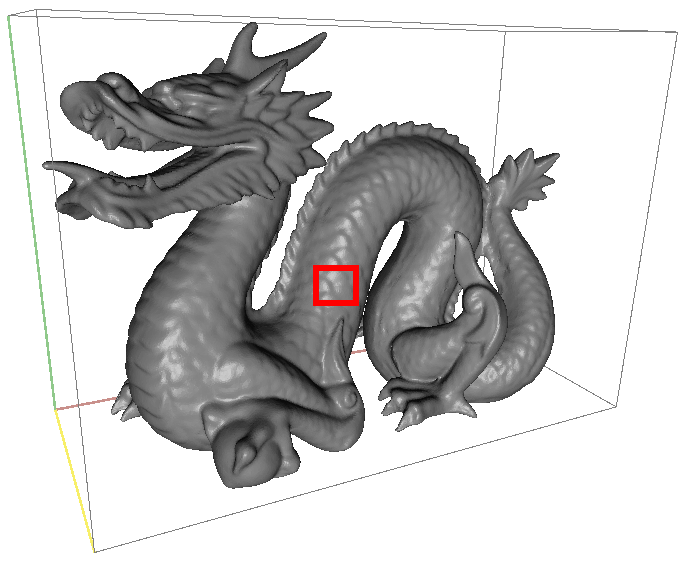
\includegraphics[scale=0.15]{pic/normal_facette-mark.png}
				% \caption{}
			\end{subfigure}
			\begin{subfigure}[b]{0.5\textwidth}
				\center
				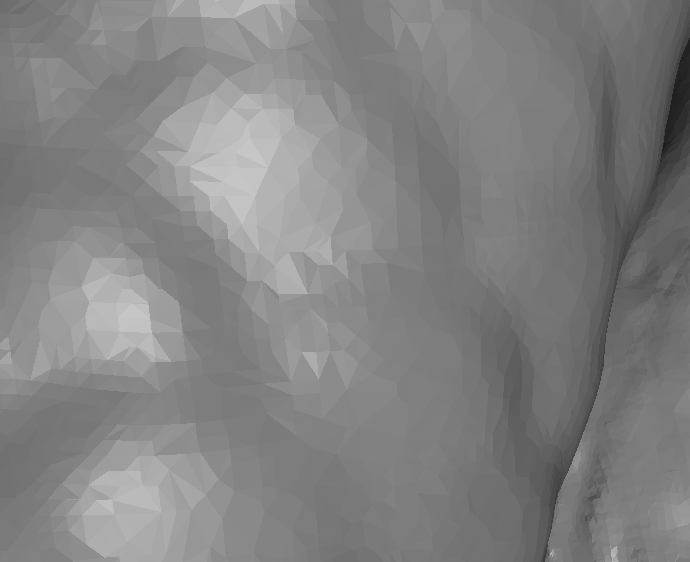
\includegraphics[scale=0.15]{pic/normal_facette-zoom.png}
				% \caption{}
			\end{subfigure}
			\caption{Die Bilder zeigen die gerenderte \enquote{Dragon}-Szene. Das rechte Bild entspricht dem roten Bereich des Linken. In dieser Szene werden die Normalen des Objektmodells durch die analytischen Normalen der Dreiecke angenähert. Da das Modell sehr fein trianguliert ist, fällt dies im ersten Bild nicht auf. Zoomt man jedoch mit der Kamera heran werden die Fehler durch die Approximation deutlich und die einzelnen Dreiecke sind mit dem menschlichen Auge auszumachen.}
			\label{fig:facette}
		\end{figure}

		Nach \cite[S.~166,~584~ff]{pbrt3} und \cite[S.~38~ff,~183~ff]{real-time-render} sind die typischen Verfahren für eine genauere Interpolation die \enquote{Vertex-Shading-Normalen} und das \enquote{Bump Mapping} (engl.: \textit{bumb mapping}).
		Formal gesehen werden bei beiden Verfahren die Normalen der vorhandenen Geometrie durch eine Normalen-Funktion ersetzt.
		\begin{figure}[h]
			\begin{subfigure}[b]{0.5\textwidth}
				\center
				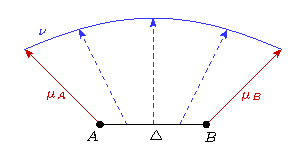
\includegraphics{gg_fig/scheme_normal-function_1.pdf}
				% \caption{Verlauf}
			\end{subfigure}
			\begin{subfigure}[b]{0.5\textwidth}
				\center
				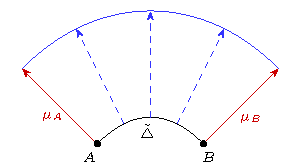
\includegraphics{gg_fig/scheme_normal-function_2.pdf}
				% \caption{approximierte Fläche}
			\end{subfigure}
			\caption{Die erste Skizze auf der linken Seite zeigt den Verlauf einer Vertex-Shading-Normalen $\nu$ anhand eines Beispiels. $A$ und $B$ sind dabei zwei Eckpunkte eines Dreiecks $\triangle$. $\mu_A$ und $\mu_B$ sind die jeweilig gegebenen Vertex-Normalen an den Eckpunkten. Im rechten Bereich der Abbildung ist die durch $\nu$ approximierte gekrümmte Fläche $\tilde{\triangle}$, auf der die Shading-Normale $\nu$ senkrecht steht, eingezeichnet.}
			\label{fig:normal-function}
		\end{figure}

		\begin{definition}[Vertex-Shading-Normale]
			Seien $\triangle$ ein Dreieck mit der Normalen $\mu$ und $\mu_A, \mu_B, \mu_C \in \shs{\mu}$ Normalen an den Eckpunkten des Dreiecks.
			Sei weiterhin $\nu$ eine Shading-Normale auf $\triangle$, sodass für alle $x\in \triangle$ mit den baryzentrischen Koordinaten $(u,v,w)$ gilt
			\[
				\nu(x) \define \frac{w\mu_A + u\mu_B + v\mu_C}{\norm{w\mu_A + u\mu_B + v\mu_C}}
			\]
			Dann ist $\nu$ stetig und man nennt es eine Vertex-Shading-Normale von $\triangle$.
		\end{definition}

		Durch das Setzen der Normalen an den Eckpunkten (engl.: \textit{vertex}) eines Dreiecks können wir sicher gehen, dass der Verlauf der Normalen stetig von einem Dreieck zu einem anderen übergeht.
		Ein beipielhafter Verlauf einer Vertex-Shading-Normalen wird in Abbildung \ref{fig:normal-function} gezeigt.
		Zu beachten ist, dass die Vektoren der Shading-Normale im Allgemeinen nicht mehr senkrecht auf der Geometrie stehen.
		Dadurch kann es, wie in \cite[S.~574~ff]{pbrt3} und \cite[S.~150~ff]{veach-thesis} gezeigt, zu Artefakten bei der Generierung des Bildes kommen.

		Der letzte Schritt zur vollständigen Beschreibung der Szenengeometrie, besteht darin, eine Menge von Dreiecken zu bilden, sodass diese ein physikalisches Objekt gut genug approximieren.
		In \cite{pbrt3} und \cite{course-triangle-mesh} werden solche Mengen auch \enquote{Meshs} (engl.: \textit{triangle mesh}) genannt.
		Wir wollen hier eine unübliche Definition geben.
		\begin{definition}[Mesh]
			Seien $n\in\SN$ und Dreiecke $\triangle_i$ mit Shading-Normalen $\nu_i$ für alle $i\in\SN,i\leq n$.
			Weiterhin definieren wir
			\[
				\e{T}\define \bigcup_{i=1}^n \triangle_i \qquad \e{A}\define \set[{ \exists!\ i\in\SN,i\leq n\colon\ x\in\triangle_i }]{x\in\e{T}}
			\]
			\[
				\func{\nu}{\e{T}}{\ssp\cup\set{0}},\qquad \nu(x)\define \sum_{i=1}^n \nu_i(x)\mathds{1}_{\e{A}\cap\triangle_i}(x)
			\]
			Dann nennen wir $\e{T}$ eine Mesh mit Shading-Normaler $\nu$, wenn für $\sigma$-fast-alle $x\in\e{T}$ auch $x\in\e{A}$ gilt.
		\end{definition}

		Die Definition der Mesh verbietet, dass die Schnittpunkte der Dreiecke eine eigene Fläche im Raum bilden.
		So können wir sicher gehen, dass die Integration über die Punkte der Mesh eine eindeutige Lösung ergibt.
		Es ist jedoch erlaubt, dass sich Dreiecke in einem Punkt oder einer Strecke schneiden dürfen.
		Dies ist auch nötig, um komplexere Objekte formen zu können.
		In der Praxis ist die genannte Bedingung im Allgemeinen erfüllt und folglich auch keine fundamentale Einschränkung \cite{pbrt3,course-triangle-mesh,surface-triangle-mesh,veach-thesis}.

	% subsection szenengeometrie (end)

	\subsection{Streuung von Licht an Oberflächen} % (fold)
	\label{sub:bsdf}

		Im letzten Abschnitt wurden die Grundbausteine einer Szene eingeführt, die deren Geometrie beschreiben.
		Wie bereits erwähnt, benötigen wir jedoch zusätzlich die Informationen, auf welche Art und Weise Licht mit den Oberflächen der Objekte interagiert.
		Dieses Verhalten wird durch die sogenannte \enquote{Bidirektionale Streuungsverteilungsfunktion} (engl.: \textit{bidirectional scattering distribution function}, BSDF), die sich aus einer \enquote{Bidirektionalen Reflektanzverteilungsfunktion} (engl.: \textit{bidirectional reflectance distribution function}, BRDF) und einer \enquote{Bidirektionalen Transmissionsverteilungsfunktion} (engl.: \textit{bidirectional transmittance distribution function}, BTDF) zusammensetzt, geklärt.
		Strukturierte Einführungen zu diesem Thema erhält man in \cite{pbrt3,veach-thesis,real-time-render,intro-brdf,radiosity}.
		\begin{definition}
			Sei $\mu\in\ssp$ die Normale am Punkt einer Oberfläche.
			Dann ist eine BSDF bezüglich $\mu$ gegeben durch eine integrierbare Abbildung $\func{f}{\ssp\times\ssp}{[0,\infty)}$ mit den folgenden Eigenschaften.

			\begin{enumerate}[label = \normalfont{(\roman*)}]
				\item
				Für $\sigma^2$-fast-alle $(\omega_\m{i},\omega_\m{o})$ mit $\omega_\m{i}\in\ssp$, $\omega_\m{o}\in\shs{\nu}$ und $\nu\define\sign(\dotp{\mu}{\omega_\m{i}})\cdot\mu$ gilt
				\[
					f(\omega_\m{i},\omega_\m{o}) = f(\omega_\m{o},\omega_\m{i}) \hfill \text{(Helmholtz-Reziprozität)}
				\]

				\item
				Für $\sigma$-fast-alle $\omega_\m{i}\in\ssp$ gilt
				\[
					\integral{\ssp}{}{f(\omega_\m{i},\omega) \abs{\dotp{\mu}{\omega}}}{\sigma(\omega)} \leq 1 \hfill \text{(Energieerhaltung)}
				\]
			\end{enumerate}
		\end{definition}

		Eine BSDF $f$ gibt an, welcher Anteil des einfallenden Lichtes aus der Richtung $\omega_\m{i}\in\ssp$ in die Richtung $\omega_\m{o}\in\ssp$ gestreut wird.
		Gilt dabei $\omega_\m{o}\in\shs{\nu}$, so befindet sich $\omega_\m{o}$ in der gleichen Hemisphere bezüglich $\mu$ wie $\omega_\m{i}$ und es handelt sich um eine Reflexion des Lichtes.
		Der verbleibende Fall beschreibt die Transmission.
		Die BSDF stellt damit eine Verallgemeinerung der idealen Reflexion und Brechung an Oberflächen dar.
		\cite[S.~571~ff]{pbrt3} und \cite[S.~135~ff]{veach-thesis} weisen zudem nach, dass die Helmholtz-Reziprozität nur für den reflektierten Anteil des Lichtes gilt.
		In Abbildung \ref{fig:brdf} ist das Beispiel einer typischen BSDF gezeigt, die keine Transmission des Lichtes zulässt \cite[S.~509~ff]{pbrt3}.

		\begin{figure}[h]
			\center
			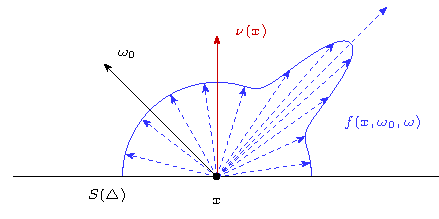
\includegraphics{gg_fig/brdf_1.pdf}
			\caption{Die Abbildung zeigt die Verteilung des reflektierten Lichtes für alle $\omega\in\shs{\mu}$ bezüglich einer konstanten Einfallsrichtung $\omega_\m{i}\in\shs{\mu}$ einer BSDF $f$ bezüglich der Oberflächennormalen $\mu\in\ssp$.}
			\label{fig:brdf}
		\end{figure}

		Die hier eingeführten Funktionen für die Charakterisierung von Materialien können auf verschiedene Weisen verallgemeinert werden.
		Zu beachten ist vor allem die fehlende Abhängigkeit von der Wellenlänge des einfallenden und der des gestreuten Lichtes, welche Effekte wie Dispersion, Irisieren und Lumineszenz verhindert.
		Eine weiteres physikalisches Phänomen stellt die Volumenstreuung dar.
		Bei der Betrachtung dieser wird ein Material durch die sogenannte \enquote{BSSRDF} beschrieben \cite[S.~671~ff]{pbrt3}.


		BSDFs sind im Allgemeinen nicht in geschlossener Form notierbar \cite[S.~507~f]{pbrt3}.
		Aus diesem Grund wollen wir für die Konstruktion realistischer Materialien wie bei der Approximation von Oberflächen verschiedene einfache BSDFs zu Grunde legen.
		In den beiden folgenden Beispielen handelt es sich um die BSDFs $f$ bezüglich der Normalen $\mu\in\ssp$ für die lambertsch diffuse Reflexion (engl.: \textit{lambertian reflection}, \cite[S.~531~f]{pbrt3}) und für die ideale Reflexion (engl.: \textit{specular reflection}, \cite[S.~144~f]{veach-thesis}).
		Weitere BSDF-Modelle sind in \cite{pbrt3,veach-thesis,radiosity} zu finden.
		Es seien $\omega_\m{i},\omega_\m{o}\in\ssp$ mit $\nu\define\sign(\dotp{\mu}{\omega_\m{i}})\cdot\mu$ gegeben.
		\[
			f(\omega_\m{i},\omega_\m{o}) = \frac{1}{\pi}\mathds{1}_{\shs{\nu}}(\omega_\m{o}) \hfill \text{(lambertsch diffuse Reflexion)}
		\]
		\[
			f(\omega_\m{i},\omega_\m{o}) = \frac{\delta_{\omega_\m{o}}(2\dotp{\mu}{\omega_\m{i}}\mu - \omega_\m{i})}{\abs{\dotp{\mu}{\omega_\m{i}}}} \hfill \text{(ideale Reflexion)}
		\]

	% subsection bsdf (end)

	\subsection{Beleuchtung und Szene} % (fold)
	\label{sub:beleuchtung_und_szene}

		Die BSDF an einem Punkt beschreibt lediglich die Streuung des einfallenden Lichtes.
		Um den Render-Verfahren einen Sinn zu geben, benötigen wir demnach Lichtquellen.
		In \cite[S.~707~ff]{pbrt3} und \cite{course-photon-map} werden verschiedene Arten von Lichtquellen definiert, implementiert und gesampled.
		Der einfachste Weg Lichtquellen einzuführen, besteht in einer abstrakten Formulierung, die unabhängig von der Szenengeometrie agiert.
		Wir wollen eine sogenannte \enquote{Umgebungsbeleuchtung} (engl.: \textit{hdr environment map} oder \textit{infinite area light}, \cite[S.~737~f]{pbrt3}) einführen.
		\begin{definition}[Umgebungsbeleuchtung]
			Eine Umgebungsbeleuchtung ist definiert als eine integrierbare Abbildung $\func{f}{(0,\infty)\times\ssp}{[0,\infty)}$.
		\end{definition}

		Diese Funktion beschreibt das Licht verschiedener Wellenlängen, welches von einer Kugeloberfläche mit quasi unendlich großem Radius in die Szene ausgesandt wird.
		Für einen Punkt der Szene, ist dessen Beleuchtung durch diese Funktion also unabhängig von dessen Position.
		Diese Tatsache wird in Abbildung \ref{fig:hdr_environment_map} wieder an einem Beispiel gezeigt.

		\begin{figure}[h]
			\center
			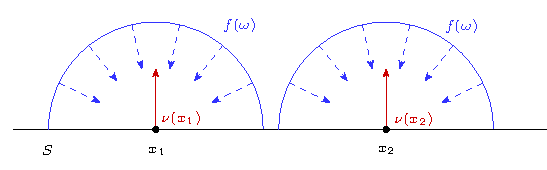
\includegraphics{gg_fig/hdr_environment_map_1.pdf}
			\caption{Die Darstellung zeigt, dass die Beleuchtung zweier Punkte $x_1$ und $x_2$ einer Oberfläche $S$ mit den Normalen $\nu(x_1)$ und $\nu(x_2)$ durch eine Umgebungsbeleuchtung $f$ nur abhängig von der Verdeckung der Punkte und nicht von deren Position ist. Bei $x_1$ und $x_2$ sind in diesem Falle die gleichen Lichtintensitäten zu messen. Es ist $\lambda\in(0,\infty)$ die Wellenlänge des Lichtes und $\omega\in\ssp$ der Raumwinkel.}
			\label{fig:hdr_environment_map}
		\end{figure}

		Aber auch die Materialien der Szene sollten in der Lage sein Licht auszusenden.
		Wir führen hierfür eine Abbildung ein, die die dafür nötigen Eigenschaften erfüllt.
		Häufig werden diese Lichtquellen auch \enquote{Feldlichtquellen} (engl.: \textit{area light}) genannt \cite[S.~733~ff]{pbrt3}.
		\begin{definition}[Emission]
			Sei $\e{T}$ eine Mesh mit einer Shading-Normalen $\nu$.
			Dann ist eine Emission von $\e{T}$ durch eine integrierbare Abbildung $\func{E}{\e{T}\times(0,\infty)\times\ssp}{[0,\infty)}$ gegeben.
		\end{definition}

		Wie bei der vorherigen Defintion beschreibt diese Funktion das ausgesandte Licht in Abhängigkeit der Wellenlänge und des Raumwinkels.
		Der Unterschied besteht darin, dass sie auf der Oberfläche einer Mesh variieren kann und sich damit auch die Beleuchtung eines Punktes je nach Position verändert.

		Durch die Einführung der Lichtquellen erhalten wir nun die vollständige Beschreibung einer Szene durch Zusammenführung der bereits definierten Strukturen.
		\begin{definition}[Szene]
			Eine Szene ist ein Tupel $(\e{T},\nu,f,E,U)$ bestehend aus einer Mesh $\e{T}$ mit einer Shading-Normalen $\nu$, einer integrierbaren Abbildung $\func{f}{\e{T}\times\ssp\times\ssp}{[0,\infty)}$, wobei $f(x,\cdot,\cdot)$ für $\sigma$-fast-alle $x\in\e{T}$ ein BSDF bezüglich $\nu(x)$ darstellt, einer Emission $E$ von $\e{T}$ und einer Umgebungsbeleuchtung $U$.
		\end{definition}


		% Für die eigentliche Approximation der Oberfläche eines Objektes benötigt man jetzt eine Menge von Primitiven.
		% Solch eine Menge wollen wir auch eine \enquote{Szene} (engl.: \textit{scene}) nennen.
		% Häufig benötigt man jedoch neben den Lichtquellen, die durch die Materialien der Primitive gegeben sind, noch weitere anders geartete Lichtquellen, die unabhängig von den eigentlichen Primitven der Szene bestehen.
		% In unserem Falle wollen wir uns speziell auf die Umgebungsbeleuchtungs-Funktion (engl.: \textit{HDR environment map}) beziehen.

		% Diese Funktion beschreibt das Licht verschiedener Wellenlängen, welches von einer Kugeloberfläche mit quasi unendlich großem Radius in die Szene ausgesandt wird.
		% Für einen Punkt der Szene, ist dessen Beleuchtung durch diese Funktion also unabhängig von dessen Position.
		% Diese Tatsache wird in Abbildung \ref{fig:hdr_environment_map} wieder an einem Beispiel gezeigt.
		% Die eigentliche Definition soll nun durch eine solche Umgebungsbeleuchtungs-Funktion erweitert werden.



	% subsection beleuchtung_und_szene (end)



	% \subsection{Szenenrepresentation} % (fold)
	% \label{sec:szenenrepresentation}

		% Um realistische Bilder zu generieren, benötigen wir als Eingabe gewisse Daten der physikalischen Objekte, die durch den Beobachter oder auch die Kamera betrachtet werden.
		% Für die später betrachteten Algorithmen ist dabei vor allem das Verhalten von Licht auf den Oberflächen dieser Objekte wichtig.
		% Der Einfachheit halber wollen wir davon ausgehen, dass das Licht nur in den oberen Schichten eines Körpers mit dessen Material wechselwirkt.
		% Für uns ist es also ausreichend, nur die Oberflächen der gegebenen Objekte und nicht deren Inneres zu beschreiben.

		% Die Oberflächen realer physikalischer Objekte sind im Allgemeinen beliebig geformt und können nicht in geschlossener Form durch eine Gleichung beschrieben werden.
		% Dennoch lassen sie sich im analytischen Sinne durch einfachere Hyperflächen im Raum approximieren.
		% Für die Bildgenerierung wählt man für solch eine Fläche meist ein Dreieck.
		% Es ist einfach zu beschreiben und flexibel genug um die meisten Objekte beliebig genau zu approximieren.
		% Dabei wollen wir entartete Dreiecke, die nur aus einem Punkt oder einer Strecke bestehen, ausschließen, da sie für die betrachteten Render-Verfahren nicht darstellbar sind.
		% \begin{definition}[Dreieck]
		% 	Ein Dreieck $\triangle$ wird durch eine Sequenz $(A,B,C)$ von Punkten in $\SR^3$, für die die Menge $\set{B-A, C-A}$ linear unabhängig ist, charakterisiert.
		% 	Seien weiterhin
		% 	\[
		% 		M \define \set[u+v\leq 1]{(u,v)\in[0,1]^2}
		% 	\]
		% 	\[
		% 		\func{\varphi}{M}{\SR^3},\qquad \varphi(u,v) \define (1-u-v)A + uB + vC
		% 	\]
		% 	Dann ist die Menge der Punkte $S$ des Dreiecks gegeben durch $\im\varphi$ und $(M,\varphi)$ stellt deren Standardparametrisierung dar.
		% 	Der Notation wegen, identifizieren wir $\triangle$ mit $S$ und definieren für alle $(u,v)\in M$
		% 	\[
		% 		\triangle(u,v) \define \varphi(u,v)
		% 	\]
		% 	Die baryzentrischen Koordinaten $(u,v,w)$ eines Punktes $x\in \triangle$ sind weiterhin durch die folgenden Eigenschaften gegeben.
		% 	\[
		% 		(u,v)\in M,\qquad w = 1-u-v,\qquad \triangle(u,v) = x
		% 	\]
		% 	Die analytische äußere Normale oder auch Normale ist definiert durch
		% 	\[
		% 		\mu \define \frac{\crossp{(B-A)}{(C-A)}}{\norm{\crossp{(B-A)}{(C-A)}}}
		% 	\]
		% \end{definition}

		% Jedes Dreieck besitzt auf seiner gesamten Fläche eine eindeutige konstante äußere analytische Normale.
		% Für die Simulation von globalen Beleuchtungseffekten ist diese Eigenschaft jedoch ein Nachteil, weil die Beleuchtung eines Objektes stark vom Verlauf seiner Normalen abhängt.
		% Nähern wir ein Objekt nun durch $n\in\SN$ Dreiecke an, so nähern wir zur Zeit auch den Normalenverlauf des Objektes durch die stückweise konstanten äußeren Normalen der Dreiecke an.
		% Der Fehler dieser Approximation tritt in Form eines facettenhaften Musters auf, welcher für das menschliche Auge gut erkennbar ist.
		% In Abbildung \ref{fig:facette} wird dieser Effekt genauer an einem Beispiel demonstriert.
		% Das Problem kann aber durch eine Interpolation, die die Stetigkeit der Normalen erhält, gelöst werden.
		% \begin{definition}[Normalen-Funktion / Shading-Normale]
		% 	Sei $\triangle$ ein Dreieck mit der Normalen $\mu$.
		% 	Dann wird $\func{\nu}{\triangle}{\shs{\mu}}$ als Normalen-Funktion oder auch Shading-Normale von $\triangle$ bezeichnet.
		% \end{definition}

		% \begin{figure}
		% 	\begin{subfigure}[b]{0.5\textwidth}
		% 		\center
		% 		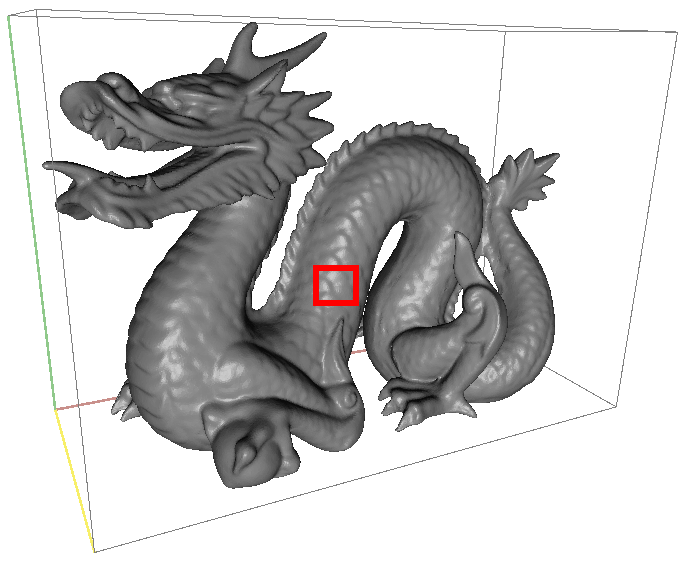
\includegraphics[scale=0.2]{pic/normal_facette-mark.png}
		% 		\caption{}
		% 	\end{subfigure}
		% 	\begin{subfigure}[b]{0.5\textwidth}
		% 		\center
		% 		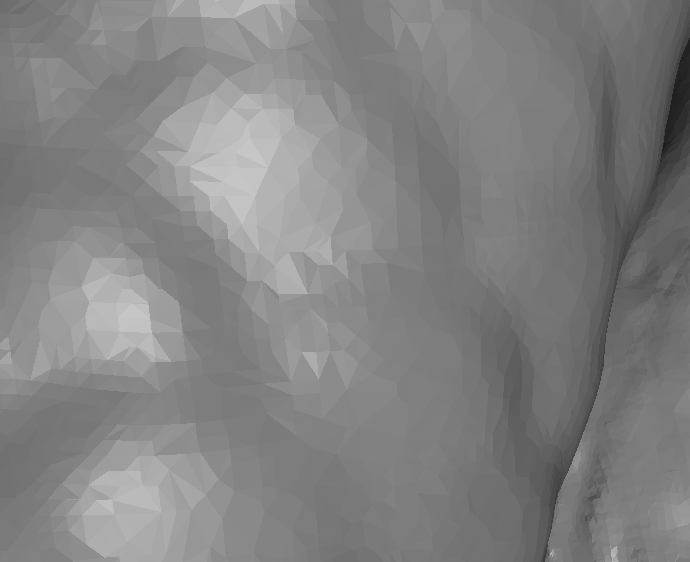
\includegraphics[scale=0.2]{pic/normal_facette-zoom.png}
		% 		\caption{}
		% 	\end{subfigure}
		% 	\caption{Die Bilder zeigen die gerenderte \enquote{Dragon}-Szene. Das rechte Bild entspricht dem roten Bereich des Linken. In dieser Szene werden die Normalen des Objektmodells durch die analytischen Normalen der Dreiecke angenähert. Da das Modell sehr fein trianguliert ist, fällt dies im ersten Bild nicht auf. Zoomt man jedoch mit der Kamera heran werden die Fehler durch die Approximation deutlich und die einzelnen Dreiecke sind mit dem menschlichen Auge auszumachen.}
		% 	\label{fig:facette}
		% \end{figure}

		% \begin{theorem}[Vertex-Shading-Normale]
		% 	Seien $\triangle$ ein Dreieck mit der Normalen $\mu$ und $\mu_A, \mu_B, \mu_C \in \shs{\mu}$ Normalen an den Punkten des Dreiecks.
		% 	Sei weiterhin $\nu$ eine Shading-Normale auf $\triangle$, sodass für alle $x\in \triangle$ mit den baryzentrischen Koordinaten $(u,v,w)$ gilt
		% 	\[
		% 		\nu(x) \define \frac{w\mu_A + u\mu_B + v\mu_C}{\norm{w\mu_A + u\mu_B + v\mu_C}}
		% 	\]
		% 	Dann ist $\nu$ stetig und man nennt es eine Vertex-Shading-Normale von $\triangle$.
		% 	% Sei $\triangle$ ein Dreieck und seien Normalen $\mu_A, \mu_B, \mu_C \in \SR^3$ an den Punkten des Dreiecks mit den folgenden Eigenschaften für alle $X\in\set{A,B,C}$ gegeben.
		% 	% \[
		% 	% 	\norm{\mu_X} = 1,\qquad \dotp{\mu_X}{\mu_\triangle} > 0
		% 	% \]
		% 	% Dann definiert die Abbildung $\func{\nu}{S(\triangle)}{\SR^3}$ eine stetige Normalen-Funktion auf $\triangle$, wenn für alle $x\in S(\triangle)$ mit den baryzentrischen Koordinaten $(u,v,w)$ die folgende Aussage gilt.
		% 	% Wir nennen $\nu$ in diesem Falle eine Vertex-Normalen-Funktion.
		% \end{theorem}

		% Durch das Setzen der Normalen an den Eckpunkten eines Dreiecks können wir sicher gehen, dass der Verlauf der Normalen stetig von einem Dreieck zu einem anderen übergeht.
		% Ein beipielhafter Verlauf einer Vertex-Normalen-Funktion wird in Abbildung \ref{fig:normal-function} gezeigt.
		% Für die in dieser Arbeit betrachteten Effekte und Verfahren reicht diese Art der Normalen-Interpolation aus.
		% Dennoch gibt es hier weitere Möglichkeiten, wie zum Beispiel \enquote{Normal Maps}, die eine noch genauere Approximation zu Lasten des Speicherverbrauchs ermöglichen.

		% \begin{figure}
		% 	\begin{subfigure}[b]{0.5\textwidth}
		% 		\center
		% 		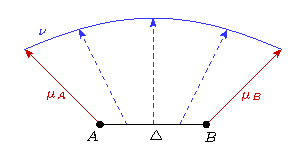
\includegraphics{gg_fig/scheme_normal-function_1.pdf}
		% 		% \caption{Verlauf}
		% 	\end{subfigure}
		% 	\begin{subfigure}[b]{0.5\textwidth}
		% 		\center
		% 		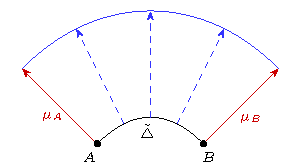
\includegraphics{gg_fig/scheme_normal-function_2.pdf}
		% 		% \caption{approximierte Fläche}
		% 	\end{subfigure}
		% 	\caption{Die erste Skizze auf der linken Seite zeigt den Verlauf einer Vertex-Normalen-Funktion $\nu$ anhand eines Beispiels. $A_\triangle$ und $B_\triangle$ sind dabei die Eckpunkte eines Dreiecks $\triangle$. $\mu_A$ und $\mu_B$ sind die jeweilig gegebenen Vertex-Normalen an den Eckpunkten. Im rechten Bereich der Abbildung ist die durch $\nu$ approximierte gekrümmte Fläche $\tilde{S}(\triangle)$, auf der die Normalen $\nu(x)$ senkrecht stehen, eingezeichnet.}
		% 	\label{fig:normal-function}
		% \end{figure}

		% Die kleinste Hyperfläche, die wir durch geschlossene Gleichungen beschreiben können und aus derer wir alle weiteren Objekte zusammensetzen, nennen wir \enquote{Primitiv} (engl.: \textit{primitive}).
		% Es soll in unserem Falle nicht nur die Informationen des Dreiecks beinhalten, sondern auch Aussagen über dessen Material oder Oberflächenstruktur treffen können.
		% Insbesondere muss das Primitiv oder dessen Material also die Reflexion, Absorbtion, Transmission und Emission des Lichts an der Oberfläche beschreiben.
		% Für physikalische Materialien gibt es aber je nach den betrachteten Effekten verschiedene verallgemeinerte Varianten der mathematischen Beschreibung.
		% Um keine dieser Varianten auszuschließen, soll hier das Primitiv in einer abstrakteren Form definiert werden.
		% \begin{definition}[Primitiv]
		% 	Sei $\s{M}$ die Menge der Elemente, die Materialien von Objekten charakterisieren.
		% 	Dann ist ein Primitiv $p$ gerade ein Tupel $(\triangle_p, \nu_p, m_p)$, bestehend aus einem Dreieck $\triangle_p$, einer Normalen-Funktion $\nu_p$ auf $\triangle_p$ und einem Material $m_p\in \s{M}$.
		% \end{definition}


		% Für die eigentliche Approximation der Oberfläche eines Objektes benötigt man jetzt eine Menge von Primitiven.
		% Solch eine Menge wollen wir auch eine \enquote{Szene} (engl.: \textit{scene}) nennen.
		% Häufig benötigt man jedoch neben den Lichtquellen, die durch die Materialien der Primitive gegeben sind, noch weitere anders geartete Lichtquellen, die unabhängig von den eigentlichen Primitven der Szene bestehen.
		% In unserem Falle wollen wir uns speziell auf die Umgebungsbeleuchtungs-Funktion (engl.: \textit{HDR environment map}) beziehen.
		% \begin{definition}[Umgebungsbeleuchtungs-Funktion]
		% 	Eine Umgebungsbeleuchtungs-Funktion ist definiert als eine integrierbare Abbildung $\func{f}{(0,\infty)\times\Omega}{[0,\infty)}$.
		% \end{definition}

		% Diese Funktion beschreibt das Licht verschiedener Wellenlängen, welches von einer Kugeloberfläche mit quasi unendlich großem Radius in die Szene ausgesandt wird.
		% Für einen Punkt der Szene, ist dessen Beleuchtung durch diese Funktion also unabhängig von dessen Position.
		% Diese Tatsache wird in Abbildung \ref{fig:hdr_environment_map} wieder an einem Beispiel gezeigt.
		% Die eigentliche Definition soll nun durch eine solche Umgebungsbeleuchtungs-Funktion erweitert werden.

		% \begin{figure}
		% 	\center
		% 	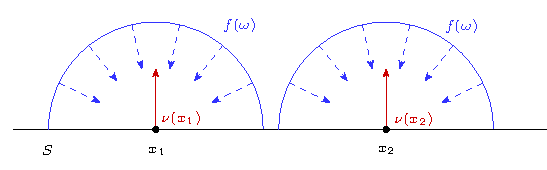
\includegraphics{gg_fig/hdr_environment_map_1.pdf}
		% 	\caption{Die Darstellung zeigt, dass die Beleuchtung zweier Punkte $x_1$ und $x_2$ einer Oberfläche $S$ mit den Normalen $\nu(x_1)$ und $\nu(x_2)$ durch eine Umgebungsbeleuchtungs-Funktion $f$ nur abhängig von der Verdeckung der Punkte und nicht von deren Position ist. Bei $x_1$ und $x_2$ sind also in diesem Falle die gleichen Lichtintensitäten zu messen.}
		% 	\label{fig:hdr_environment_map}
		% \end{figure}

		% \begin{definition}[Szene]
		% 	Eine Szene $\s{S}$ bezeichnet ein Tupel $(P_\s{S},E_\s{S})$ mit einer endlichen Menge $P_\s{S}$ von Primitiven und einer Umgebungsbeleuchtungs-Funktion $E_\s{S}$.
		% 	Die Menge $S(\s{S})$ der Punkte in der Szene $\s{S}$ sei definiert durch
		% 	\[
		% 		S(\s{S}) \define \bigcup_{p\in P_\s{S}} S(\triangle_p)
		% 	\]
		% \end{definition}

	% subsection szenenrepresentation (end)

	\subsection{Raytracing} % (fold)
	\label{sub:raytracing}

		Im einfachsten Falle bezeichnet das Wort \enquote{Raytracing} (engl.: \textit{ray tracing}) einen Algorithmus zur Ermittlung der Sichtbarkeit von dreidimensionalen Objekten bezüglich eines Ursprungpunktes (engl.: \textit{origin}) im Raum \cite{pbrt3,parker-ray-tracing}.
		Häufig versteht man darunter jedoch auch eine Render-Technik für die Generierung eines gesamten Bildes aus einer gegebenen Szene, die auf dem eben genannten Raytracing-Algorithmus basiert \cite{pbrt3, nikodym-ray-tracing, parker-ray-tracing}.

		Grundsätzlich gibt es viele Verfahren, um ein Szene auf ein Bild zu rendern \cite{survey-visibility,real-time-render}.
		Die Erfahrung zeigt aber, dass vor allem in Bereichen, in denen die globalen Beleuchtungseffekte realistisch simuliert werden sollen, Raytracing eine wichtige Grundlage darstellt.
		Der Grund dafür besteht in der Tatsache, dass Raytracing das \enquote{Sichtbarkeitsproblem} (engl.: \textit{visibility problem}, \cite{3d-visibility, survey-visibility}) löst und durch die Verwendung von Strahlen eine Basis für die Lichtberechnung im Sinne der geometrischen Optik bereitstellt \cite{pbrt3,veach-thesis,parker-ray-tracing}.
		\begin{definition}[Sichtbarkeitsproblem]
			Sei $\e{T}$ eine Mesh.
			Dann ist die Sichtbarkeitsfunktion von $\e{T}$ die folgende Abbildung.
			\[
				\func{V_\e{T}}{\SR^3\times\e{T}}{\set{0,1}}
			\]
			\[
				V_\e{T}(o,x)=
				\begin{cases}
					1 &: \e{T} \cap \set[\gamma\in(0,1)]{(1-\gamma)o + \gamma x} = \emptyset \\
					0 &: \m{sonst}
				\end{cases}
			\]
			Das Sichtbarkeitsproblem beschreibt die Aufgabe diese Funktion für gegebene Parameter zu evaluieren.
		\end{definition}

		Die Sichtbarkeitsfunktion gibt an, ob der Oberflächenpunkt $x$ vom Beobachtungspunkt $o$ aus in gerader Linie gesehen werden kann oder ob zwischen diesen Punkten ein weiterer Punkt der Mesh $\e{T}$ den Punkt $x$ verdeckt \cite[S.~30]{3d-visibility}.
		Daran anknüpfend besteht die Basis des Raytracing-Verfahrens auf dem Aussenden von \enquote{Strahlen} (engl.: \textit{ray}) bezüglich eines Ursprungspunktes \cite{pbrt3,parker-ray-tracing,nikodym-ray-tracing}.
		Für diese Strahlen kann der Schnittpunkt mit $\e{T}$ ermittelt werden.
		Liegt der Schnittpunkt zwischen $o$ und $x$, so beträgt der Wert der Sichtbarkeitsfunktion $0$.
		Im noch bleibenden Fall ergibt sich der Wert zu $1$.
		Die Sichtbarkeitsfunktion kann somit für alle gegebenen Parameter durch Raytracing berechnet werden.
		Abbildung \ref{fig:ray_tracing-1} zeigt diese Methode anhand einer Skizze.

		\begin{figure}[h]
			\center
			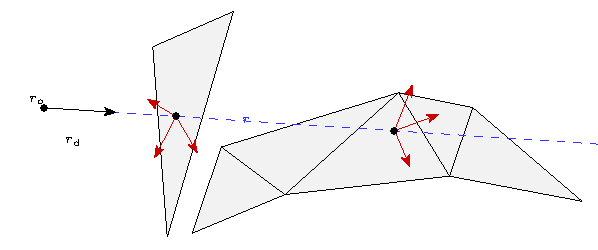
\includegraphics{gg_fig/ray_tracing_1.pdf}
			\caption{Die Abbildung zeigt eine Skizze, welche das Sichtbarkeitsproblem und den Raytracing-Algorithmus verdeutlicht. Die grau melierten Dreiecke sollen die gegebene Mesh $\e{T}$ darstellen. Der ausgesendete Strahl $r$, gegeben durch $(r_\m{o},r_\m{d})$, trifft in der Mesh genau zwei Punkte $x_1$ und $x_2$. Dabei wird $x_2$ durch $x_1$ verdeckt. Es gilt also $V_\e{T}(r_\m{o},x_1)=1$ und $V_\e{T}(r_\m{o},x_2)=0$.}
			\label{fig:ray_tracing-1}
		\end{figure}

		% \begin{definition}[Strahl]
		% 	Ein Strahl $r$ sei gerade durch ein Tupel $(r_\m{o},r_\m{d})$ mit einem Ursprungspunkt $r_\m{o}\in\SR^3$ und einer Richtung $r_\m{d}\in\SR^3\setminus\set{0}$ charakterisiert. Die Menge $S(r)$ der Punkte des Strahls ist gegeben durch das Bild der Parametrisierung $([0,\infty),\varphi_r)$
		% 	\[
		% 		S(r) \define \im{\varphi_r},\qquad \func{\varphi_r}{[0,\infty)}{\SR^3},\qquad \varphi_r(t)\define r_\m{o} + tr_\m{d}
		% 	\]
		% 	Die Menge aller Strahlen sei mit $R$ bezeichnet.
		% \end{definition}

		\begin{definition}[Strahl]
			Seien ein Ursprung $o\in\SR^3$, eine Richtung $d\in\ssp$ und die folgende Abbildung gegeben.
			\[
				\func{\varphi}{[0,\infty)}{\SR^3},\qquad \varphi(\gamma)\define o + \gamma d
			\]
			Dann wird das Bild $\im\varphi$ ein Strahl $r$ genannt.
			Dabei ist $([0,\infty),\varphi)$ die Standardparametrisierung von $r$.
			Der Notation wegen, definieren wir für alle $\gamma\in[0,\infty)$
			\[
				r(\gamma) \define \varphi(\gamma)
			\]
			Durch das Tupel $(o,d)$ charakterisieren und identifizieren wir den Strahl $r$.
			Die Menge aller Strahlen definieren wir als $\e{R}$.
		\end{definition}

		Die vollständige Evaluierung von $V_\e{T}$ ist jedoch häufig nicht notwendig.
		In Abbildung \ref{fig:ray_tracing-1} ist klar, dass alle Punkte von $r$, die hinter $x_1$ liegen von dem Beobachtungspunkt $r_\m{o}$ aus nicht sichtbar sind.
		Beim eigentlichen Raytracing-Algorithmus wirkt sich diese Eigenschaft positiv aus.
		Es reicht für eine gegebene Richtung und einen gegebenen Beobachtungspunkt den nächsten Schnittpunkt des resultierenden Strahles zu ermitteln.
		Für alle weiteren Schnittpunkte, sofern diese existieren, ergibt sich die Sichtbarkeitsfunktion zu Null, wodurch sie für das weitere Vorgehen ignoriert werden können \cite[S.~4~ff,~866]{pbrt3}.
		\begin{definition}[Raytracing-Funktion]
			Sei $\e{T}$ eine Mesh.
			Dann ist die Raytracing-Funktion von $\e{T}$ durch die folgende Abbildung gegeben.
			\[
				\func{\m{rt}_\e{T}}{\e{R}}{(0,\infty]}
			\]
			\[
				\m{rt}_\e{T}(r) \define
				\begin{cases}
					\min\set[r(\gamma)\in \e{T}]{\gamma\in(0,\infty)} &: \e{T}\cap (r\setminus\set{r(0)}) \neq \emptyset \\
					\infty &: \m{sonst}
				\end{cases}
			\]
		\end{definition}

		Wie bereits erwähnt, erweitert man diesen Algorithmus häufig mit der Berechnung eines gesamten Bildes, indem man für jeden Pixel des Bildes einen oder mehrere Strahlen durch einen analogen virtuellen Pixel im Szenenraum schießt und die Raytracing-Funktion für diese evaluiert \cite{pbrt3,parker-ray-tracing,nikodym-ray-tracing}.
		Abbildung \ref{fig:ray_tracing-2} zeigt dieses Verfahren anhand einer Skizze.
		\begin{figure}[h]
			\center
			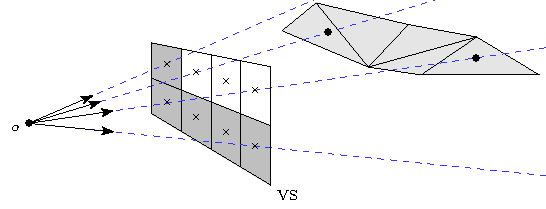
\includegraphics{gg_fig/ray_tracing_2.pdf}
			\caption{In der Skizze ist ein typisches Render-Verfahren auf der Basis des Raytracing-Algorithmus dargestellt. Bezüglich eines Beobachtungspunktes $o\in\SR^3$ wird durch jeden Pixel eines virtuellen Bildschirms $\m{VS}$ ein Strahl geschossen und der Wert der Raytracing-Funktion evaluiert. Die grau melierten Dreiecke bilden die Mesh $\e{T}$. Je nachdem, ob ein Strahl einen Schnittpunkt mit $\e{T}$ aufweist, wird ein entsprechendes Shading-Verfahren ausgeführt. Der Übersicht wegen sind im Bild nur vier der eigentlich acht Strahlen sichtbar.}
			\label{fig:ray_tracing-2}
		\end{figure}
		Um gleichzeitig das sogenannte \enquote{Shading} zu ermöglichen, ermittelt man nicht nur den Schnittpunkt, sondern auch in welchem Dreieck sich dieser befindet und welche baryzentrischen Koordinaten er besitzt \cite{pbrt3,ray-triangle-intersection}.
		Die Implementierung des Raytracing-Verfahrens soll hier nicht gezeigt werden, da eine einfache Implementierung einen zu großen Rechenaufwand darstellt und die hier verwendete optimierte Variante weit über das Thema dieser Arbeit hinausgeht.
		Für eine strukturierte Einführung von Beschleunigungsstrukturen sei auf \cite[S.~247~ff]{pbrt3} und \cite{parker-ray-tracing,nikodym-ray-tracing} verwiesen.

	% subsection raytracing (end)

	\subsection{Radiometrie} % (fold)
	\label{sub:radiometrie}

		Ein physikalischer Körper $K$ mit der Oberfläche $\partial K$ und äußerer Normalen-Funktion $\mu$ sendet aufgrund verschiedener physikalischer Effekte, wie zum Beispiel Reflexion oder Emission, elektromagnetische Wellen aus \cite{nolting-edyn}.
		Für die Simulation von Beleuchtungseffekten ist es nötig die Abhängigkeit dieser Abstrahlung für verschiedene Wellenlängen $\lambda\in(0,\infty)$, verschiedene Oberflächenpunkte $x\in\partial K$ und verschiedene Richtungen $\omega\in\ssp$ zu betrachten.
		Dafür führen wir die sogenannte \enquote{spektrale Strahldichte} (engl.: \textit{spectral radiance}) ein.
		Sie gibt an, wie viel Energie pro Zeit, pro Wellenlängenänderung, pro Flächenelement und pro Raumwinkel abgestrahlt beziehungsweise empfangen wird \cite{intro-radiometry,malacara-colorimetry,ohta-colorimetry}.
		Sind also messbare Teilmengen $\Lambda\subset (0,\infty)$, $U\subset \partial K$ und $S\subset\ssp$ gegeben, so kann man die spektrale Strahldichte über die abgegebene Strahlungsleistung $\Phi(U,\Lambda,S)$ der Oberfläche $U$ in den Raumwinkelbereich $S$ definieren \cite{intro-radiometry}.
		Die zugehörige Abbildung ist dann wie folgt gegeben.
		\[
			\func{\s{L}}{\partial K\times(0,\infty)\times \ssp}{[0,\infty)}
		\]
		\[
			\Phi(U,\Lambda,S) \definedby \integral{U}{}{ \integral{\Lambda}{}{ \integral{S}{}{ \s{L}(x,\lambda,\omega)\abs{\dotp{\mu(x)}{\omega}} }{\sigma(\omega)} }{\lambda(\lambda)} }{\sigma(x)}
		\]
		Abbildung \ref{fig:radiance} zeigt eine Skizze, welche die Struktur dieser Abbildung verdeutlicht.
		Der Erfahrung nach stellt die spektrale Strahldichte für das menschliche Auge die sinnvollste messbare Größe für die empfundene Helligkeit einer Oberfläche bezüglich eines Beobachtungspunktes dar \cite{malacara-colorimetry,ohta-colorimetry}.

		\begin{figure}[h]
			\center
			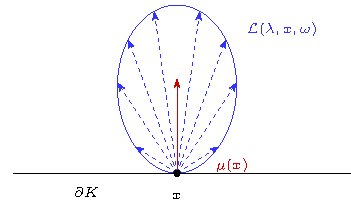
\includegraphics{gg_fig/radiance_1.pdf}
			\caption{Die Skizze stellt das qualitative Beispiel einer spektralen Strahldichte $\s{L}$ dar, die an einem Punkt $x$ auf der Oberfläche $\partial K$ mit der äußeren Normalen $\mu$ und für eine Wellenlänge $\lambda$ eine Verteilung in Abhängigkeit von $\omega\in\ssp$ besitzt.}
			\label{fig:radiance}
		\end{figure}

		Eine weitere Größe, die wir hier einführen möchten, ist die sogenannte spektrale \enquote{Bestrahlungsstärke} oder auch spektrale Irradianz (engl.: \textit{spectral irradiance}).
		Sie wird vor allem bei der noch folgenden Konstruktion der Irradiance Maps benötigt werden.
		Wir definieren sie für eine messbare Teilmenge $S\subset\ssp$ \cite[S.~9~f]{guide-radiometry}.
		\[
			\func{\s{E}}{\partial K\times (0,\infty)}{[0,\infty)},\qquad \s{E}(x,\lambda) \define \integral{S}{}{ \s{L}(x,\lambda,\omega)\abs{\dotp{\mu(x)}{\omega}} }{\sigma(\omega)}
		\]
		Die spektrale Bestrahlungsstärke quantifiziert die Energie pro Zeit, pro Wellenlängenänderung und pro Flächenelement, die an einem Punkt auf der Oberfläche des Objektes aus dem Raumwinkelbereich $S$ empfangen wird \cite{intro-radiometry,guide-radiometry}.

		Für die weiteren Algorithmen und Implementierungen reicht es entkoppelte Abbildungen zu betrachten, welche für jeden Punkt einer Szene und jede gegebene Richtung der Strahldichte beziehungsweise der Irradianz entsprechen.
		Später werden dies die Funktionen sein, die wir durch \enquote{Path Tracing} simulieren und durch geeignetes \enquote{Surface Caching} zwischenspeichern wollen.
		\begin{definition}[Strahldichte und Irradianz]
			Sei $\Sigma\define (\e{T},\nu,f,E,U)$ eine Szene.
			Dann ist eine Strahldichte von $\Sigma$ gegeben durch eine integrierbare Abbildung
			\[
				\func{L}{\e{T}\times(0,\infty)\times\ssp}{[0,\infty)}
			\]
			Die zu $L$ gehörige Irradianz definieren wir durch die folgende Funktion.
			\[
				\func{E}{\e{T}\times(0,\infty)}{[0,\infty)},\qquad E(x,\lambda)\define \integral{\shs{\nu(x)}}{}{L(x,\lambda,\omega)\dotp{\mu(x)}{\omega}}{\sigma(\omega)}
			\]
		\end{definition}

	% subsection radiometrie (end)



	% \subsection{Reflexionen an Oberflächen} % (fold)
	% \label{sub:reflexionen_an_oberflächen}

	% 	\begin{definition}
	% 		Sei $\mu\in\ssp$ eine Normale.
	% 		Dann ist eine BSDF bezüglich $\mu$ gegeben durch eine integrierbare Abbildung
	% 		\[
	% 			\func{f}{\ssp\times\ssp}{[0,\infty)}
	% 		\]
	% 		mit den folgenden Eigenschaften.

	% 		\begin{enumerate}[label = \normalfont{(\roman*)}]
	% 			\item Für alle $\omega_\m{i},\omega_\m{o}\in\shs{\mu}$ und $\tilde{\omega}_\m{i},\tilde{\omega}_\m{o}\in\shs{-\mu}$
	% 			\[
	% 				f(\omega_\m{i},\omega_\m{o}) = f(\omega_\m{o},\omega_\m{i})\qquad f(\tilde{\omega}_\m{i},\tilde{\omega}_\m{o}) = f(\tilde{\omega}_\m{o},\tilde{\omega}_\m{i}) \hfill \text{(Helmholtz-Reziprozität)}
	% 			\]
	% 			\item \label{item:brdf_energy_conservation} $\integral{\ssp}{}{f(\omega,\omega_\m{o}) \abs{\dotp{\mu}{\omega}}}{\sigma(\omega)} \leq 1 \hfill \text{(Energieerhaltung)}$
	% 		\end{enumerate}
	% 	\end{definition}

	% 	Um Primitive zu definieren nutzten wir eine abstrakte Menge $\s{M}$, welche die Elemente enthielt, die die Materialien unserer Szene charakterisierten.
	% 	Der Grund dafür war, dass die Beschreibung von Materialien ein komplexes Thema ist, dessen vollständige Behandlung hier nicht möglich ist.
	% 	Wir wollen uns hier auf eine spezielle Kategorie von Materialen beschränken.
	% 	Dabei beachten wir nur die Reflexion und Absorbtion, nicht aber die Transmission von Licht.
	% 	Die Idee besteht darin, ein Material durch eine geeignete Funktion auf der Oberfläche zu charakterisieren.
	% 	Diese Funktionen nennt man \enquote{Bidirektionale Reflektanzverteilungsfunktionen} (engl.: \textit{bidirectional reflectance distribution function}, BRDF).
	% 	Sie beschreiben den Anteil des reflektierten Lichtes in Abhängigkeit des Ein- und Ausfallwinkels.
	% 	In Abbildung \ref{fig:brdf} wird anhand einer Skizze die folgende Definition Dieser verdeutlicht.
	% 	\begin{definition}[BRDF]
	% 		Sei $\mu\in\Omega$ eine Normale.
	% 		Dann ist eine BRDF bezüglich $\mu$ gegeben durch eine integrierbare Abbildung
	% 		\[
	% 			\func{f}{\Theta_\mu\times\Theta_\mu}{[0,\infty)}
	% 		\]
	% 		Es handelt sich bei $f$ um eine physikalische BRDF, wenn die folgenden Eigenschaften für alle $\omega_\m{i},\omega_\m{o}\in\Theta_\mu$ erfüllt sind.
	% 		\begin{enumerate}[label = \normalfont{(\roman*)}]
	% 			\item $f(\omega_\m{i},\omega_\m{o}) = f(\omega_\m{o},\omega_\m{i}) \hfill \text{(Helmholtz-Reziprozität)}$
	% 			\item \label{item:brdf_energy_conservation} $\integral{\Theta_\mu}{}{f(\omega_\m{i},\omega) \abs{\dotp{\mu}{\omega}}}{\sigma(\omega)} \leq 1 \hfill \text{(Energieerhaltung)}$
	% 		\end{enumerate}
	% 		Gilt in \ref{item:brdf_energy_conservation} die Gleichheit, so nennt man $f$ auch eine ideale physikalische BRDF.
	% 	\end{definition}

	% 	\begin{figure}
	% 		\center
	% 		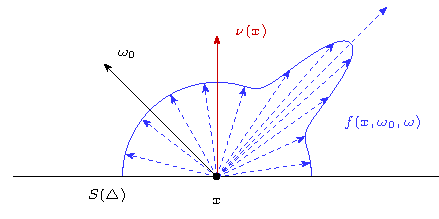
\includegraphics{gg_fig/brdf_1.pdf}
	% 		\caption{Die Abbildung zeigt die typische Verteilung des reflektierten Lichtes über der Hemisphere einer häufig verwendeten BRDF $f$ bezüglich einer konstanten Einfallsrichtung $\omega_0$ an einem Punkt $x\in S(\triangle)$. Auch hier sind $\triangle$ ein Dreieck und $\nu$ eine Normalen-Funktion auf $\triangle$.}
	% 		\label{fig:brdf}
	% 	\end{figure}

	% 	BRDFs sind im Allgemeinen nicht in geschlossener Form notierbar.
	% 	Aus diesem Grund wollen wir für die Konstruktion realistischer BRDFs verschiedene einzelne Reflexionsmodelle zu Grunde legen.
	% 	Die daraus entstehenden idealen BRDFs können dann durch eine Linearkombination miteinander verbunden werden, um so reale Materialien nachzuahmen.
	% 	Zu beachten ist, dass die beiden folgenden eingeführten Beispiele solcher Modelle gewisse auftretende physikalische Effekte, wie zum Beispiel die Fresnel-Reflexion, nicht berücksichtigen.
	% 	\begin{definition}[spezielle BRDFs]
	% 		Sei $\mu\in\Omega$ eine Normale.
	% 		Dann definiert man die folgenden BRDFs bezüglich $\mu$ für alle $\omega_\m{i},\omega_\m{o}\in\Theta_\mu$.
	% 		\begin{enumerate}[label = \normalfont{(\roman*)}]
	% 			\item $\m{ldr}(\omega_\m{i},\omega_\m{o}) \define \frac{1}{\pi} \hfill \text{(lambertsch diffus)}$
	% 			\item $\m{psr}(\omega_\m{i},\omega_\m{o}) \define \frac{1}{\abs{\dotp{\mu}{\omega_\m{i}}}} \delta_{\omega_\m{o}}(2\dotp{\mu}{\omega_\m{i}}\mu - \omega_\m{i}) \hfill \text{(perfekt spiegelnd)}$
	% 		\end{enumerate}
	% 	\end{definition}

	% 	Möchte man zusätzlich die Transmission von Licht an einem Punkt mit Normaler $\mu\in\Omega$ betrachten, so lässt sich analog zur Menge der BRDFs bezüglich $\mu$ eine Menge von Funktionen auf $\Theta_{-\mu}\times\Theta_{-\mu}$ definieren.
	% 	Die Funktionen dieser Klasse werden \enquote{Bidirektionale Transmissionsverteilungsfunktionen} (engl.: \textit{bidirectional transmittance distribution function}, BTDF) genannt.
	% 	Die Zusammenführung einer BRDF und einer BTDF auf $\Omega$ führt zur verallgemeinerten \enquote{Bidirektionalen Streuungsverteilungsfunktion} (engl.: \textit{bidirectional scattering distribution function}, BSDF).


	% subsection reflexionen_an_oberflächen (end)

	\subsection{Rendergleichung} % (fold)
	\label{sub:rendergleichung}

		Die \enquote{Rendergleichung} (engl.: \textit{rendering equation} oder \textit{light transport equation}, \cite[S.~861]{pbrt3}) ist eine Integralgleichung, die 1986 von James T. Kajiya entwickelt wurde, um die bis zu diesem Zeitpunkt verbreiteten Rendertechniken für die Simulation globaler Beleuchtungseffekte auf eine gemeinsame Basis zu stellen \cite{kajiya-lte}.
		In \cite{kajiya-lte}, \cite[S.~349~ff,~862~ff]{pbrt3} und \cite{veach-thesis} wird sie mithilfe der Prinzipien der geometrischen Optik und dem Energieerhaltungssatz hergeleitet.
		\cite{veach-thesis} stellt dabei die resultierende Gleichung zusätzlich in einer Operator-Formulierung dar.
		Insbesondere handelt es sich bei der Rendergleichung um eine Fredholm-Integralgleichung 2.Art, die unter gewissen Voraussetzungen eine eindeutige Lösung besitzt (siehe hierzu \cite[S.~103~ff]{veach-thesis} und \cite{integral-equations}).
		% \begin{definition}[Rendergleichung]
		% 	Sei $\s{S}$ eine gegebene Szene mit Strahldichte-Funktion $L_\s{S}$.
		% 	Dann gehorcht $L_\s{S}$ der Rendergleichung, wenn für alle $x\in S(\s{S})$ und $\omega_0\in \Omega$ gilt
		% 	\begin{alignat*}{3}
		% 		L_\s{S}(x,\omega_0) &= E_\s{S}(x,\omega_0) \\
		% 		&+\Integral{S(\s{S})}{}{ V_\s{S}(x,y) G_\s{S}(x,y) f_\s{S}(x,\omega(x,y),\omega_0) L_\s{S}(y,\omega(x,y)) }{\sigma(y)}
		% 	\end{alignat*}
		% 	Der Übersicht halber wurden dabei die folgenden Symbole verwendet.
		% 	\[
		% 		G_\s{S}(x,y) \define \frac{\abs{\dotp{\nu(x)}{\omega(x,y)}}\abs{\dotp{\nu(y)}{\omega(x,y)}}}{\norm{x-y}^2}\qquad \omega(x,y) \define \frac{y-x}{\norm{y-x}}
		% 	\]
		% 	Aufgrund der komplexen Struktur verwenden wir auch eine weitere Variante.
		% 	\[
		% 		L_\s{S}(x,\omega_0) = E_\s{S}(x,\omega_0) + \integral{\Omega}{}{ f_\s{S}(x,\omega,\omega_0)\tilde{L}_\s{S}(x,\omega) \abs{\dotp{\nu(x)}{\omega}} }{\sigma(\omega)}
		% 	\]
		% \end{definition}

		\begin{definition}
			Seien $\Sigma\define (\e{T},\nu,f,E,U)$ eine Szene und $L$ eine Strahldichte von $\Sigma$.
			Dann gehorcht $L$ der Rendergleichung, wenn für alle $x\in\e{T}$, $\lambda\in(0,\infty)$ und $\omega_\m{o}\in\ssp$ das Folgende gilt.
			\[
				L(x,\lambda,\omega_\m{o}) = E(x,\lambda,\omega_\m{o}) + \integral{\ssp}{}{ f(x,\omega,\omega_\m{o})\tilde{L}(x,\lambda,\omega) \abs{\dotp{\nu(x)}{\omega}} }{\sigma(\omega)}
			\]
			\[
				\tilde{L}(x,\lambda,\omega)\define
				\begin{cases}
					L(r(\m{rt}_\e{T}(r)),\lambda,-\omega) &: r\in\e{R}, r\equiv(x,\omega),\ \m{rt}_\e{T}(r) < \infty \\
					U(\lambda,\omega) &: \m{sonst}
				\end{cases}
			\]
		\end{definition}

		In der Definition entspricht $\tilde{L}(x,\lambda,\omega)$ der aus $\omega$ einfallenden Strahldichte am Punkt $x$ der Wellenlänge $\lambda$.
		Die Funktionen $\tilde{L}$ und $L$ sind über die Raytracing-Funktion miteinander verbunden.
		Existiert jedoch für den gegebenen Strahl $r$ kein Schnittpunkt mit der Szene, so entspricht die einfallende Strahldichte gerade der Umgebungsbeleuchtung.
		In Abbildung \ref{fig:lte-incident-emitted-radiance} wird dieser Zusammenhang an einem Beispiel demonstriert.
		Die Strahldichte in Richtung $\omega$ entspricht damit der Summe des emittierten und des gestreuten Lichtes am Punkt $x$.

		\begin{figure}[h]
			\center
			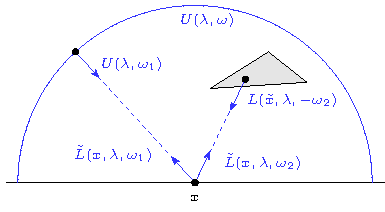
\includegraphics{gg_fig/lte-incident_and_emitted_radiance.pdf}
			\caption{Die Abbildung skizziert an einem Beispiel die Relation der Funktionen $L$ und $\tilde{L}$ aus der Definition der Rendergleichung. Dabei stellen das Dreieck einen Teil der Mesh, $U$ die Umgebungsbeleuchtung für $\omega\in\ssp$, $\omega_1,\omega_2$ Raumrichtungen, $\lambda$ die betrachtete Wellenlänge und $x$ einen Punkt auf der Mesh dar. Für $\tilde{x}$ gilt nach Defintion $\tilde{x}=r(\m{rt}_\e{T}(r))$, wobei der Strahl $r$ durch $(x,\omega_2)$ gegeben ist. Der Strahl in Richtung $\omega_1$ besitzt keinen Schnittpunkt mit der Szene, wodurch sich die einfallende Strahldichte aus der Umgebungsbeleuchtung ergibt.}
			\label{fig:lte-incident-emitted-radiance}
		\end{figure}

		Gehorcht die Strahldichte einer Szene der Rendergleichung, so simuliert sie die globalen Beleuchtungseffekte dieser Szene auf einer physikalischen Basis, wodurch die entstehenden Lichtverhältnisse für das menschliche Auge real wirken \cite{kajiya-lte,pbrt3,veach-thesis}.
		Die Rendergleichung lässt sich aber im Allgemeinen nicht analytisch lösen \cite{pbrt3,veach-thesis,kajiya-lte}.
		% In \cite[S.~863~f]{pbrt3} ist jedoch die Lösung eines Spezialfalls beschrieben.
		Aus diesem Grund sind verschiedene numerische Lösungsmethoden für die Berechnung einer Strahldichte, die der Rendergleichung gehorcht, entwickelt worden.
		Die berühmtesten Beispiele stellen das \enquote{Path Tracing} \cite{kajiya-lte}, das \enquote{Bidirectional Path Tracing} \cite{bidirectional-path-tracing}, der \enquote{Metropolis Light Transport} \cite{veach-mlt} und das \enquote{Photon Mapping} \cite{course-photon-map} dar.
		Eine strukturierte Einführung zu diesen Verfahren gibt es auch hier in \cite{pbrt3}.
		Das Beispiel für eine durch Path Tracing erzeugte Lösung ist in Abbildung \ref{fig:example-audi-r8-pt} zu sehen.

		\begin{figure}[h]
			\center
			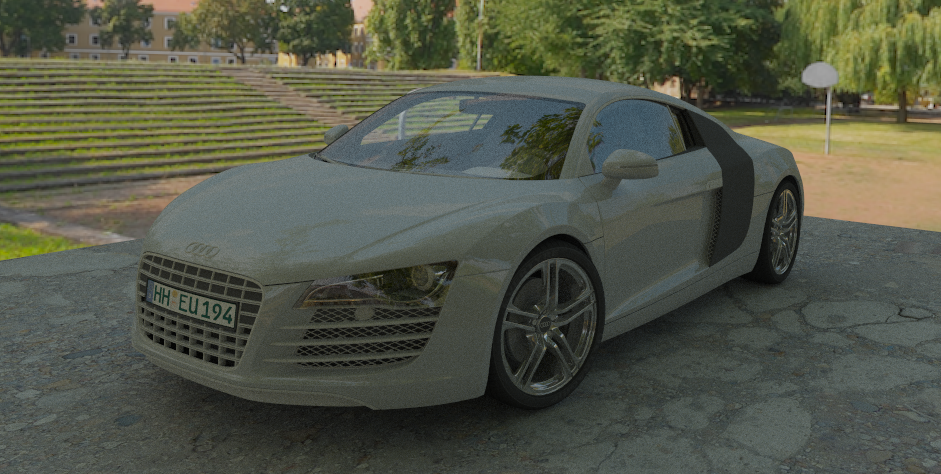
\includegraphics[scale=0.4]{pic/example-audi_r8-pt.png}
			\caption{Die Abbildung stellt eine durch Path Tracing simulierte Lösung der Rendergleichung für die \enquote{Audi R8}-Szene dar. Die Lichtquelle besteht hier alleine aus der Umgebungsbeleuchtung. Für die BSDFs ist immer eine Mischung aus idealer Reflexion, lambertsch diffuser Reflexion und idealer Brechung gewählt worden.}
			\label{fig:example-audi-r8-pt}
		\end{figure}

		Alle genannten Verfahren arbeiten auf der Basis von Zufallszahlen.
		Da die Rendergleichung eine mehrdimensionale Integralgleichung ist, bietet sich die Verwendung verschiedener \enquote{Monte-Carlo-Methoden} an \cite{monte-carlo-method}.
		Für uns bedeutet diese Tatsache, dass es sich bei der Abfrage der Strahldichte für diese numerischen Verfahren um die Realisierung einer Zufallsvariable handelt, deren Erwartungswert im besten Falle der der wahren Strahldichte entspricht.
		Eine detailliertere Betrachtung dieser Eigenschaft wird in den weiteren Kapiteln folgen.
		Für die Konstruktion der Irradiance Maps ist es im Grunde genommen unwichtig, welcher Algorithmus verwendet wird, sofern er in der Lage ist die Strahldichte für gegebene Parameter zu evaluieren.
		Wir verwenden hier einen einfachen Path Tracing Algorithmus.

	% subsection rendergleichung (end)

	% \subsection{Surface Caching} % (fold)
	% \label{sub:surface_caching}

	% 	Der Begriff \enquote{Surface Caching} (deutsch: \textit{Oberflächenpuffer}) wurde vor allem durch das Computerspiel \enquote{Quake} geprägt.
	% 	Es war das erste Spiel welches sogenannte \enquote{Surface Caches} und Lightmaps verwendete, um so die grafischen Berechnungen während der Laufzeit auf ein Minimum zu beschränken.
	% 	Der Begriff selbst ist nicht standardisiert und wird meistens verwendet um Algorithmen, die in der \enquote{Quake-Engine} vorkommen, genauer zu erläutern.
	% 	Wir wollen diesen Begriff für eine Oberklasse von Algorithmen und Datenstrukturen verwenden, die es entweder ermöglichen Informationen auf Oberflächen einer Szene zu speichern oder diese Informationen aus einem geeigneten Oberflächenpuffer wieder auszulesen.
	% 	Insbesondere wollen wir uns mit dem Speichern von Strahldichten diffuser Lichtverteilungen beschäftigen, bei denen die Strahldichte-Funktion $L$ nur vom Ort der Szene und nicht mehr vom betrachteten Raumwinkel abhängt.

	% 	Zu beachten ist, dass die hier genannten Verfahren im Allgemeinen nur für statische Szenen Sinn ergeben, da eine Veränderung der Geometrie und Lichtverhältnisse dazu führt, dass der Surface Cache keine aktuellen Informationen mehr enthält.
	% 	Er müsste demnach bei jeder Änderung der Szene neu berechnet werden.
	% 	Da die betrachteten Szenen teilweise sehr groß sein können, wäre dieser Schritt ineffizient.
	% 	Zwei typische Verfahren zum zwischenspeichern von Strahldichten werden in den beiden folgenden Unterabschnitten genauer erläutert.

	% 	\subsubsection{Vertex Lighting} % (fold)
	% 	\label{sub:vertex_lighting}

	% 		Bei der Implementierung einer Szene $\s{S}$ haben wir Vertices eingeführt, um die Speicherkosten von $\s{S}$ zu verringern.
	% 		Dabei existiert jeder Vertex unabhängig von allen Primitiven.
	% 		Nur die Primitive besitzen die Informationen, aus welchen Vertices sie selbst bestehen.
	% 		Dies führt zu der Idee, die diffuse Strahldichte-Funktion $L_\s{S}$ an den Positionen aller Vertices zu evaluieren und zu speichern.
	% 		Möchte man dann die Szene rendern, so kann man für jeden Strahl, der ein Schnittpunkt $x$ mit der Szene hat, das getroffene Primitiv $p$ und die zugehörigen baryzentrischen Koordinaten $(u,v,w)$ des Schnittpunktes bestimmen.
	% 		Die Strahldichte an dieser Position wird dann durch die folgende Gleichung interpoliert.
	% 		\[
	% 			L_\s{S}(x,\cdot) \approx w L^{(0)}_\s{S}g + u L^{(1)}_\s{S} + v L^{(2)}_\s{S}
	% 		\]

	% 		Es handelt sich hierbei um Gourad-Shading oder auch bilineare Interpolation auf dem Dreieck.

	% 	% subsubsection vertex_lighting (end)

	% 	\subsubsection{Lightmap} % (fold)
	% 	\label{ssub:lightmap}

	% 		\urldef{\urllightmapexample}\url{https://upload.wikimedia.org/wikipedia/commons/1/15/Lightmapped_Scene_with_Lightmap.png}

	% 		Lightmaps sind Datenstrukturen, welche vorberechnete Helligkeitswerte für Oberflächen einer Szene in einer Textur speichern.
	% 		Damit sind sie vor allem für Anwendungen, die sich extrem auf die Grafikkarte des Computers stützen, geeignet, da Grafikkarten speziell eingebaute Hardware besitzen, um Texturen zu verarbeiten.
	% 		Der gesamte Prozess der Generierung und Nutzung einer solchen Datenstruktur wird auch \enquote{Lightmapping} genannt.
	% 		Abbildung \ref{fig:lightmap-example}\footnote{Quelle: \urllightmapexample \\ Donnerstag 27.April 17.20 Uhr} zeigt ein einfaches Beispiel.

	% 		\begin{figure}[h]
	% 			\center
	% 			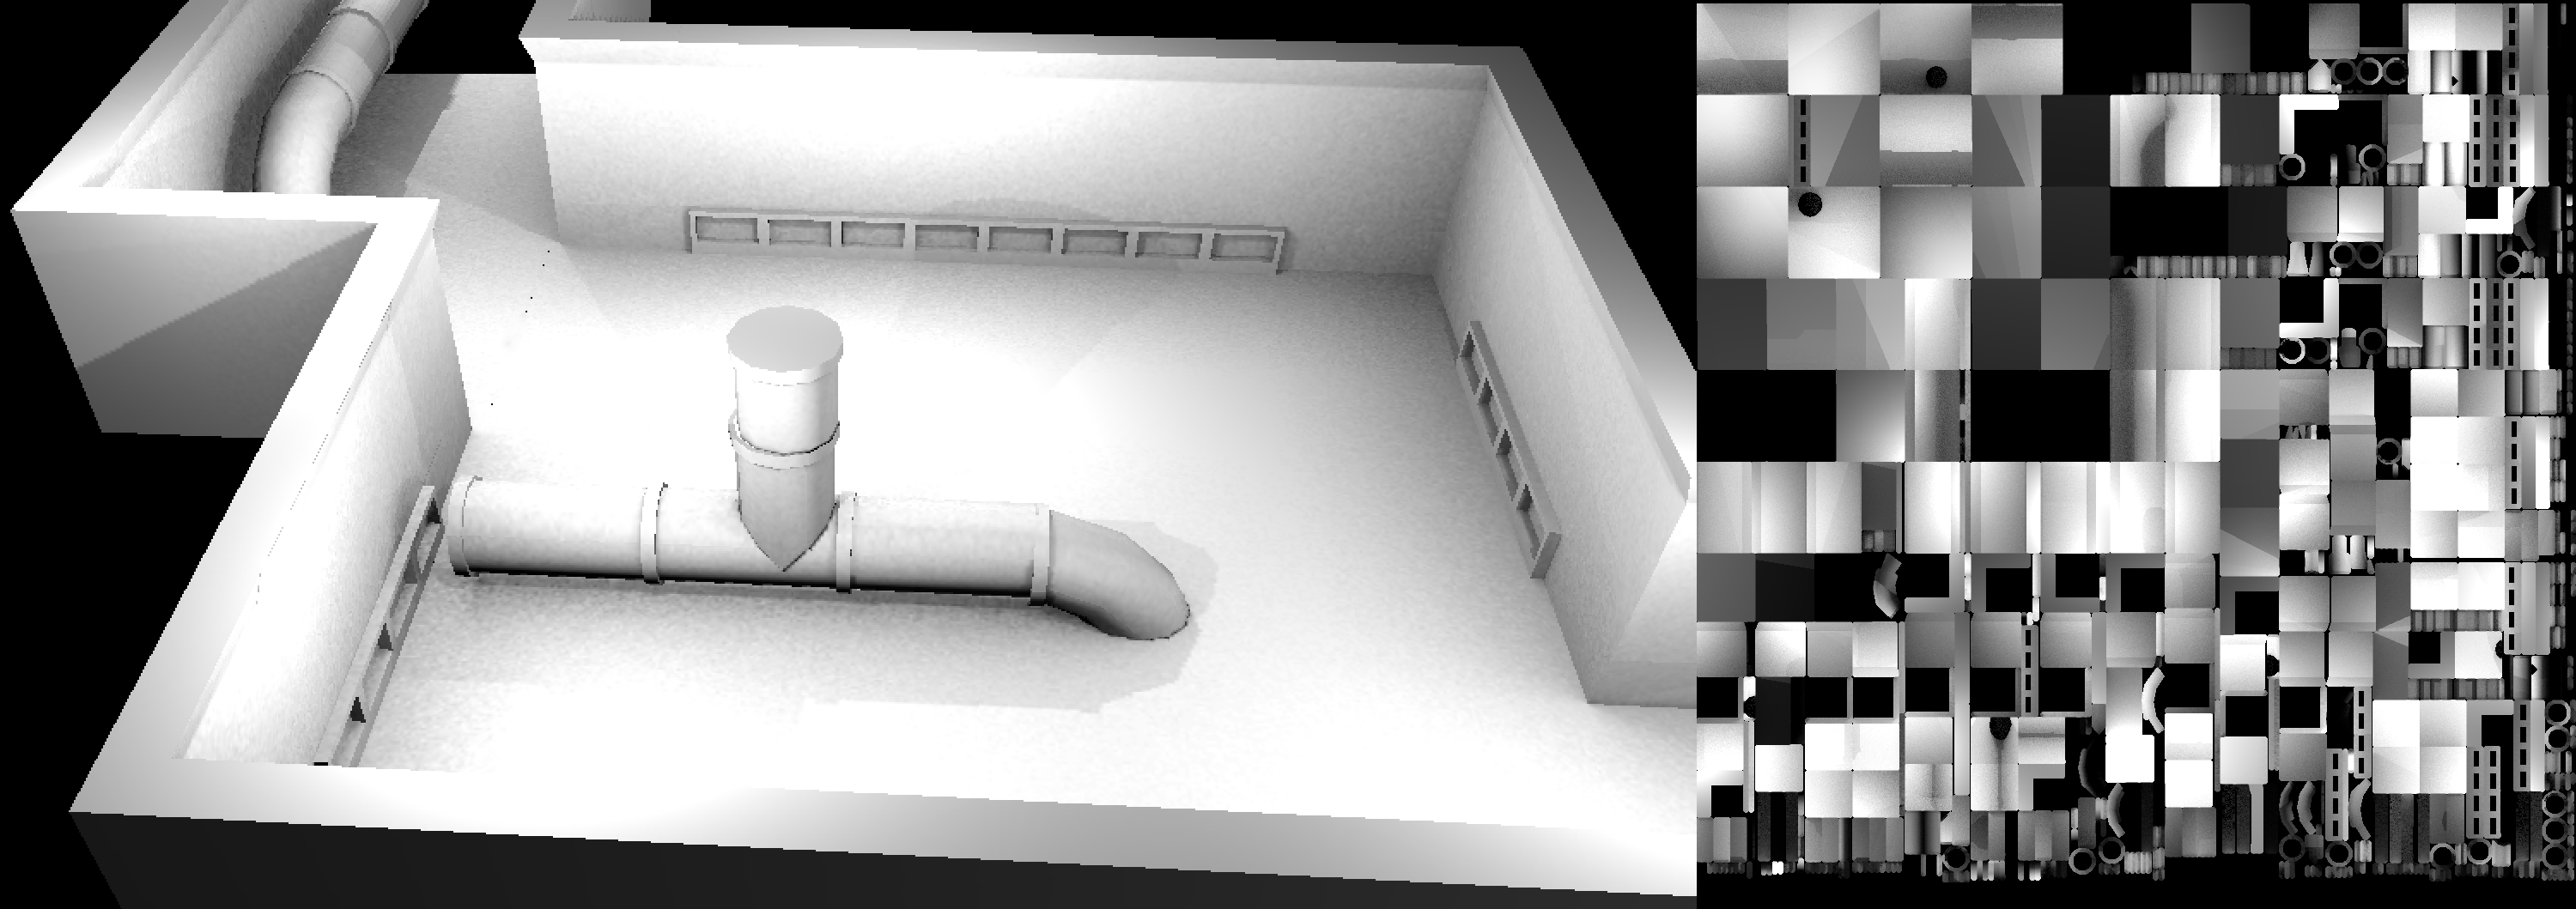
\includegraphics[scale=0.2]{pic/lightmap_example.png}
	% 			\caption{Die rechte Seite der Abbildung zeigt ein typisches Beispiel einer Lightmap-Textur. Mit ihrer Hilfe kann im linken Bereich des Bildes die Szene \enquote{gelightmapped} werden. Beim eigentlichen Rendern der Szene sind nun keine Sichtbarkeitstests mehr nötig, um Schatten zu generieren.}
	% 			\label{fig:lightmap-example}
	% 		\end{figure}

	% 		Lightmaps werden im Allgemeinen manuell optimiert, um den speziellen Gegebenheiten einer Szene gerecht zu werden.
	% 		Dies erfordert eine Menge zusätzlichen Zeit- und Arbeitsaufwand, sobald eine neue Szene betrachtet werden soll.
	% 		Lightmaps besitzen außerdem auch alle Nachteile von Texturen.
	% 		Die Größe der Speicher heutiger Grafikkarten ist im Vergleich zu den normalen Arbeitsspeichern eher gering.
	% 		Damit ist natürlich auch die Größe der Lightmap beschränkt.
	% 		Ein weiterer Nachteil ist, dass sich eine Textur, die quadratische Pixel besitzt, niemals vollständig an ein Dreieck in der Szene anpassen kann.
	% 		Die Folge ist, dass bei zu dicht gelegenen Helligkeitswerten auf der Lightmap, die zu verschiedenen Dreiecken gehören, Interpolations-Artefakte auftreten.

		% subsubsection lightmap (end)

	% subsection surface_caching (end)

% section grundlagen_und_methoden (end)

	\newpage

	\begin{figure}[h]
		\center
		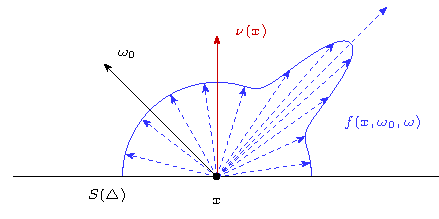
\includegraphics{gg_fig/brdf_1.pdf}
		\caption{}
	\end{figure}

	Diese Definition zeigt diverse Probleme auf, die bei der Modellierung von Objekten entstehen können.
	Dreiecke der Primitive in einer Szene dürfen sich im Allgemeinen beliebig schneiden.
	Dadurch ist es im Allgemeinen nicht möglich jedem Oberflächenpunkt eine eindeutige äußere Normale zuzuordnen.
	Bei der Generierung der Irradiance Maps werden sich diese Punkte als Fehler äußern.

	Die abstrakte Definition ist für die Implementierung leider noch nicht ausreichend.

	\begin{figure}[h]
		\center
		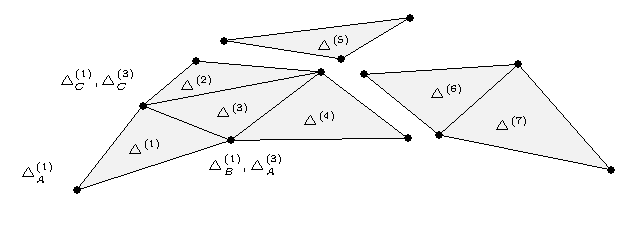
\includegraphics{gg_fig/triangle_mesh_1.pdf}
		\caption{Die Abbildung zeigt eine beispielhafte Menge von Dreiecken $\set[i\in\SN,i\leq 7]{\triangle^{(i)}}$. Verschiedene Gruppen von Dreiecken bilden eine Approximation einer Oberfläche im Raum. Dabei werden die Eckpunkte der Dreiecke geteilt und es gilt zum Beispiel $\triangle^{(1)}_B=\triangle^{(3)}_A$ und $\triangle^{(1)}_C = \triangle^{(3)}_C$.}
		\label{fig:triangle_mesh}
	\end{figure}



\end{document}